\documentclass[a4paper, 12pt]{report}

\usepackage[utf8]{inputenc}
\usepackage[ngerman]{babel}
\usepackage[T1]{fontenc}
\usepackage{amsmath}
\usepackage{braket}
\usepackage{amssymb}
\usepackage{graphicx}
\usepackage{wrapfig}
\usepackage{hyperref}
\usepackage{float} 
\usepackage{lmodern}
\usepackage{cleveref}
\usepackage{blindtext}

\author{Sebastian Steinhäuser}

\begin{document}

\renewcommand{\thepage}{\roman{page}}% Roman page numbers
\begin{center}
	\Large{\textbf{Masterarbeit}}
	\\
	\vspace{1cm}
	\Huge{\textbf{Computersimulation wechselwirkender aktiver Teilchen anhand eines Gittermodells}}
	\\
	\vspace{1cm}
	\Large{Sebastian Steinhäuser}
	
\includegraphics[width=0.75\textwidth]{DLR.jpg}
\end{center}
\begin{center}
	Betreut durch Thomas Voigtmann und Julian Reichert
\end{center}
\newpage
\tableofcontents
\clearpage

\chapter{Einleitung}
\renewcommand{\thepage}{\arabic{page}}\setcounter{page}{1}
Die Bewegung aktiver Teilchen ist in verschiedensten Bereichen, sowie \break Schnittstellen zwischen, der Physik, Biologie und Medizin nach wie vor von hohem Interesse. Modelle aktiver Teilchen helfen das mikroskopischen Verhalten von Zellen oder Bakterien zu erklären. Weitere Beispiele um aktive Materie auf makroskopischer Ebene zu Beobachten sind Fisch- und Vogelschwärme.
\\
\noindent Gittermodelle spielen eine große Rolle in der computergestützen Physik, da ihre diskrete Struktur ideal in Programme für den Computer umgewandelt werden kann ohne vorher noch 'künstlich' diskretisiert zu werden, wie es beim numerischen lösen von (partiellen) Differentialgleichungen oder ähnlichem der Fall ist. Desweiteren lassen sich Gittermodelle einfach formulieren und kommen oft mit wenigen Parametern, mit intuitiver Bedeutung, aus. Es entstehen so einfache abstrakte Modelle für aktive Teilchen, zum Beispiel lassen sich Staus und Warteschlangen anhand des TASEP-Modell erklären ('totally asymmetric simple exclusion process')\cite{Derrida_1993} Gittermodelle, wie zum Beispiel der TASEP, werden häufig anhand sogenannter Monte-Carlo-Simulationen (kurz: MC) untersucht. 
\\
\noindent Die Idee der Monte-Carlo-Simulation ist es durch ziehen von Zufallszahlen einen analytisch schwer oder unmöglich berechenbaren Zustandsraum zu samplen. So kannte Beispielsweise Georges-Louis Leclerc, Comte de Buffon schon im Jahre 1777 die Kreiszahl $\pi$ über die wohl erste durchgeführte Monte-Carlo-'Simulation' bestimmen. Buffon lies dabei Nadeln fixer Länge auf ein liniertes Papier fallen und zählte wieviele Nadeln die Linien schneiden. Für die Wahrscheinlichkeit, dass eine Nadel die Linie schneidet exisiert eine analytische Formel. Buffon konnte also anhand dieser Formel und aus dem Verhältnis von 'Treffern' zu 'Versuchen' die Kreiszahl $\pi$ bestimmen\cite{Buffon}. 
\\
\noindent Knapp 200 Jahre später und mit der Hilfe von Computern nutzen Nicholas Metropolis, Arianna W. Rosenbluth, Marshall N. Rosenbluth, Augusta H. Teller und Edward Teller die Idee der Monte-Carlo-Simulation unter zur Hilfenahme der 'detailed balance' für ihre berühmte Arbeit über die Zustandsgleichung harter Kugeln (Scheiben) in zwei Dimensionen\cite{doi:10.1063/1.1699114}. Diese Arbeit hatte schnell Verallgemeinerungen auf weitere Dimensionen und Lennard-Jones-Systemen\cite{doi:10.1063/1.462271} zur Folge und brachte einen enormen Fortschritt im Bereich der Flüssigkeiten.
Ein berühmtes Beispiel für ein mit Monte-Carlo-Simulation untersuchtes Gittermodell ist der 'selbstmeidende-Pfad', auch: 'self-avoiding-walk' (SAW) genannt. Anhand von Computersimulation diser SAW's (in drei Dimensionen) konnte die in der Polymerphysik bekannte Florryexponent für die 'power-law' zwischen der Anzahl an Monomere und der End-to-End Länge des Polymer $\nu = \frac{3}{5}$ auf $\nu \approx 0.585$ korregiert werden\cite{Grassberger_1993}. Der SAW gibt genau den sogennaten 'excluded volume' Effekt wieder, denn zwei Monomere können sich nicht an der selben Stelle befinden.
\\
\noindent Perkolierende Cluster waren in den 70er und 80er Jahren stark diskutierte Themen, da so Phänomene wie die elektrische Leitfähigkeit von Legierungen, Ausbreitungen von Epidemien und Waldbränden beschrieben werden können \cite{Wiki_Perkolationstheorie}, sowie poröse medien nachgestellt werden können\cite{doi:10.1063/1.4999485}. Der Random-Walk auf dem perkolierenden Cluster ist ein Modell welches die Diffusion in porösen Medien erlären kann. Es tritt sogenannte 'anormale' Diffusion\cite{PhysRevLett.50.77} auf, also ein nicht-triviales Potenzgesetz für das $msd$ (mittlere quadratische Verschiebung).
\\
\noindent Die statistische Physik bietet zudem die Möglichkeit auch auf völlig andere neue Gebiete/Bereiche angewendet zu werden, in diesem Fall wird das PAC-MAN Spiel der 80er Jahre mit Methoden der (computergestützten) statistischen Physik untersucht\cite{doi:10.1063/1.4999485}, genauer: anhand von Monte-Carlo-Simulation. Ein weiteres schönes Beispiel wo statistische Physik 'zweckentfremdet' angewendet werden kann ist das allseits bekannte Schachspiel, auch hier können Aussagen über einen ansonsten unüberschaubar großen Zustandsraum (die Stellung der Figuren) getroffen werden\cite{Atashpendar_2016}.
\\
\noindent In dem 'Clearing out a maze'-Paper\cite{doi:10.1063/1.4999485} wird ein Modell für einen biased Random-Walk, bei dem zuvor unbesuchte Felder mit einer bestimmtem Parameter (der sogenannten 'Nahrungspropensität') unterschiedlich stark bevorzugt werden, auf dem perkolierenden Cluster untersucht und als Chemotaxis in porösen Medien interpretiert.
\\
\noindent Ergebniss dieser Arbeit ist, dass dieses Modell eine anormale Diffusion mit einem neuen (zuvor in aktiver un passiver Mikroschwimmerdynamik unbekannten), von der Nahrungspropensität abhängigen, Exponenten für das $msd$-Potenzgesetz hervorruft. Es wurde gefunden, dass der Diffusionsexponent mit steigender Nahrungspropensität abnimmt, wohingegen ein Walk dieser Art auf dem freien Gitter (ohne Hindernisse) sich schneller ausbreiten würde.
\\
\noindent In dieser Arbeit wuidme ich mich der Frage, wie mehrere 'PAC-MAN'-Walker durch gegenseitiges 'wegfressen' von Nahrung sich beeinflussen. Diese durch 'Chemotaxis' induzierte dynamische Wechselwirkung zwischen den Walkern wird sowohl auf dem freien Gitter als auch wie in \cite{doi:10.1063/1.4999485} auf dem perkolierenden Cluster mittels Monte-Carlo-Simulation untersucht.


\chapter{Perkolation}
\section{Was ist Perkolation?}
In dieser Arbeit geht es um Perkolation und vor allem um den Random-Walk (mathematisches Modell für eine Bewegung, bei der die einzelnen Schritte zufällig erfolgen) auf einem perkolierenden Cluster in einem Quadratgitter in zwei Raumdimensionen. In diesem Fall gibt es zwei geläufige Perkolationsmodelle, Knotenperkolation (engl. 'site-percolation') und Kantenperkolation (engl. 'bond-percolation'), hier wird immer über Knotenperkolation gesprochen. In folgender Abbildung wird der Unterschied zwischen Knoten- und Kantenperkolation bildlich dargestellt \cite{Wiki_Perkolationstheorie}.
\begin{figure}[h!]
	\centering
	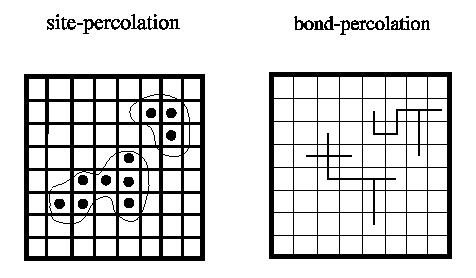
\includegraphics[scale=0.6]{Percolation1.jpg}
	\caption{Knoten- und Kantenperkolation}
\end{figure}
\vspace{0,5cm}
\\
Das Quadratgitter wird zufällig mit einer Wahrscheinlichkeit $1-p$ geblockt. Es ist Konvention, die Wahrscheinlichkeit, dass ein Platz frei ist, mit $p$ zu bezeichnen, diese Konvention möchte ich hier erhalten. Geblockte Plätze können nicht besetzt werden. Man kann sich geblockte Plätze wie Wände eines Labyrinths vorstellen, durch die der Random-Walker später nicht hindurch kommt.  
\\
Nun definiert man einen Cluster als eine Gruppe benachbarter Quadrate die begehbar sind, also nicht geblockt. Man nennt einen Cluster perkolierend, wenn sich der Cluster von einer Kante zur gegenüberliegenden Kante erstreckt, so dass zum Beispiel Wasser durch das Gitter fließen könnte, ähnlich wie es durch eine Kaffeemaschiene (engl. 'percolator') perkoliert/sickert. Vereinfacht gesagt kann ein Random-Walker auf dem perkolierenden Cluster sich unendlich ausbreiten und ist nicht 'eingesperrt'. Man kann sich nun leicht Vorstellen, dass wenn kaum Felder geblockt sind (also $p$ nahe $1$) sich auf dem (unendlich großen) Quadratgitter stets ein perkolierender Cluster finden lässt und wenn kaum Felder begehbar sind (also $p$ nahe $0$) sich nie ein perkolierender Cluster finden lässt. Es gibt dazwischen eine sogenannten kritischen Wert $p=p_c \approx 0.5928$ \cite{Stauffer} bis zu welchem das unendliche Quadratgitter perkoliert, auch Perkolationsschwelle oder englisch percolation-threshold genannt.
\noindent Historisch geht die Perkolationstheorie (engl. 'percolation theory') auf Paul Flory und Walter H. Stockmayer zurück, die sie während des Zweiten Weltkriegs entwickelten, um Polymerisationsprozesse zu beschreiben. Der Polymerisationsprozess kommt durch das Aneinanderreihen von Molekülen zustande, die dadurch Makromoleküle bilden. Der Verbund solcher Makromoleküle führt zu einem Netzwerk von Verbindungen, die sich durch das ganze System ziehen können.\cite{Wiki_Perkolationstheorie}
\\
\noindent Üblicherweise wird der Beginn der Perkolationstheorie mit einer Publikation von Broadbent  und Hammersley aus dem Jahre 1957 in Verbindung gebracht, in welcher der Name eingeführt wurde, und in welcher sie mit den oben erläuterten geometrischen und wahrscheinlichkeitstheoretischen Konzepten mathematischer behandelt wurde. Hammersley erwähnt in seiner persönlichen Geschichte der Perkolation in 'Percolation Structures and Processes', dass die (damals) neuen Computer, die für die Wissenschaftler dieser Zeit zugänglich wurden, einer der Gründe für die Entwicklung der Perkolationstheorie waren: Hier handelte es sich um Probleme, bei denen die Computer nützlich werden konnten.

\section{Perkolation auf dem Computer}
Es ist selbstverständlich nicht möglich ein unendlich großes Quadratgitter mit zufällig geblockten und freien Gitterplätzen auf dem Computer zu erzeugen, daher wird hier stets ein endliches Quadratgitter (auf dem Computer in Form einer Matrix/Array gespeichert) und mit periodischen Randbedingungen ausgestattet. Um perkolierende Cluster dieser zufällig erzeugten Matrix zu finden nutzt man den sogenannten Hoshen-Kopelmann-Algorithmus.\cite{Fricke}
Dieser Algorithmus lässt sich am besten an einem Beipiel erklären. Im nachfolgenden Bild sind freie Felder grau und geblockte Felder weiß, graue Felder die an einer Kante verbunden sind (wo der Random-Walker also von einem Feld ins andere kann) werden mit dem selben Label versehen.
\begin{figure}[h!]
	\centering
	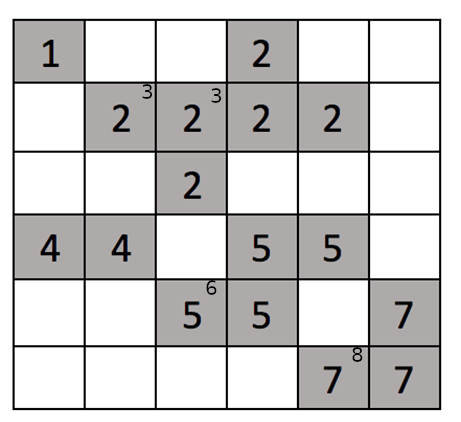
\includegraphics[scale=0.5]{H-K_algorithm.png}
	\caption{Veranschaulichung des Hoshen-Kopelmann-Algorithmus. Die 'alten' Labels stehen, falls unterschiedlich vom Label, oben in der rechten Ecke.}
\end{figure}

\newpage
\subsection{Implementierung des Hoshen-Kopelmann-Algorithmus}
Die Idee, wie man dieses anschauliche Nummerieren auf den Computer überträgt ist es, die Matrix von (zum Beispiel) oben links beginnend abzugehen. Stößt man auf ein begehbares Feld (also einen Eintrag $1$ in der Matrix) vergleicht man mit dem Label über und links von diesem Feld, haben beide das selbe Label, so wird dieses auch in das Feld, welches aktuell bearbeitet wird, eingetragen; haben die beiden Felder ein unterschiedliches Label, so merkt man sich in einer Liste, dass diese beiden Label jetzt verbunden sind durch das aktuell zu bearbeitende Feld und später zusammengefügt werden müssen. Sind die Felder oben und links von dem zu bearbeitenden Feld geblockt, so labelt man das Feld mit dem nächst größeren noch nicht benutzten Label. Ist man in diesem Verfahren durch die Matrix durch, so fügt man die verlinkten Labels zusammen; es gilt als Konvention das kleinst mögliche Label zu verwenden. Zum Beispiel verlinkt das vierte Feld der zweiten Reihe in obiger Abbildung 2 die Labels 2 und 3 oder das vierte Feld der fünften Reihe die Labels 5 und 6.
\noindent In python ist dieser Algorithmus für das Labeling (welcher auch in der Bildverarbeitung genutzt wird) bereits in der $scipy.ndimage$ Bibliothek als $measurements$ vorhanden. Nachfolgende Grafik zeigt einen Pseudocode\cite{Fricke} des Hoshen-Kopelmann-Algorithmus, man kann schön die Unterteilung in scannen des Clusters, verlinken von Labeln (union) und finden der Equivalenzklasse (des Labels) (find) sehen.\newpage

\begin{figure}
	\centering
	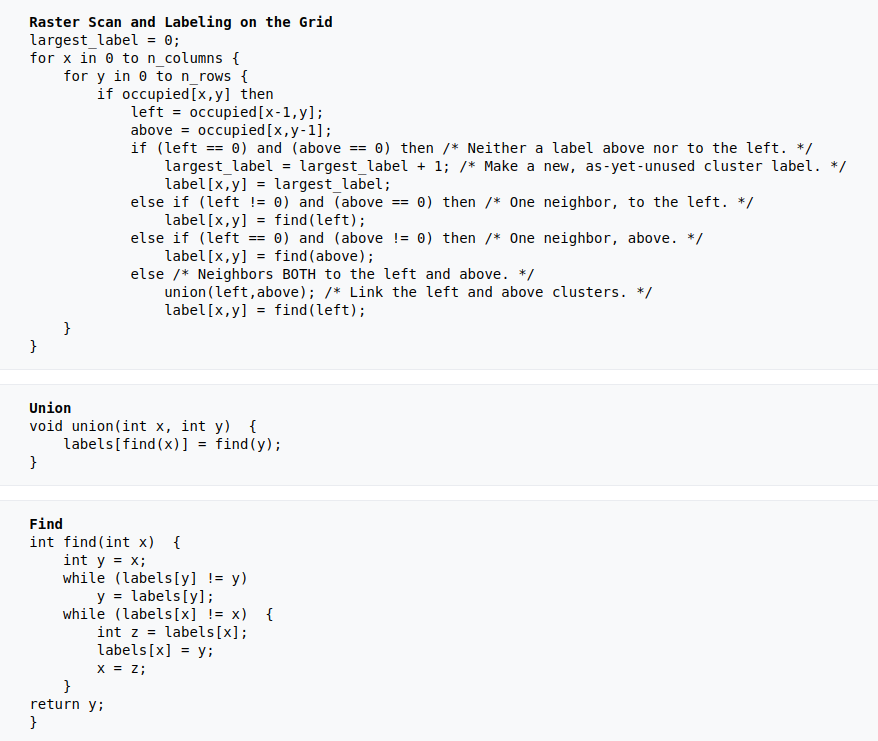
\includegraphics[scale=0.7]{HSK_pseudocode.png}
	\caption{Pseudocode des Hoshen-Kopelmann-Algorithmus}
\end{figure}

\clearpage
\subsection{Finden von gerichtet perkolierender \label{gerichtet}}
Geht ein Cluster von einem Rand zum gegenüberliegenden Rand, also tritt an diesen beiden Kanten das selbe Label auf so perkoliert dieser Cluster in der endlichen Matrix. Durch die periodischen Randbedingungen muss das Label am gegenüberliegenden Rand in der gleichen 'Höhe' auftreten. Es wird also einfach der linke Rand der Matrix abgegangen und das jeweilige Label mit dem Label an dem rechten Rand verglichen. Analog verfährt man mit dem oberen Rand. Diese Möglichkeit der Perkolation ist durch die periodischen Randbedingungen allerdings nicht die einzige, wie das nächste Unterunterkapitel zeigt.

\subsection{Diagonal perkolierende Cluster}
\begin{figure}[h!]
	\centering
	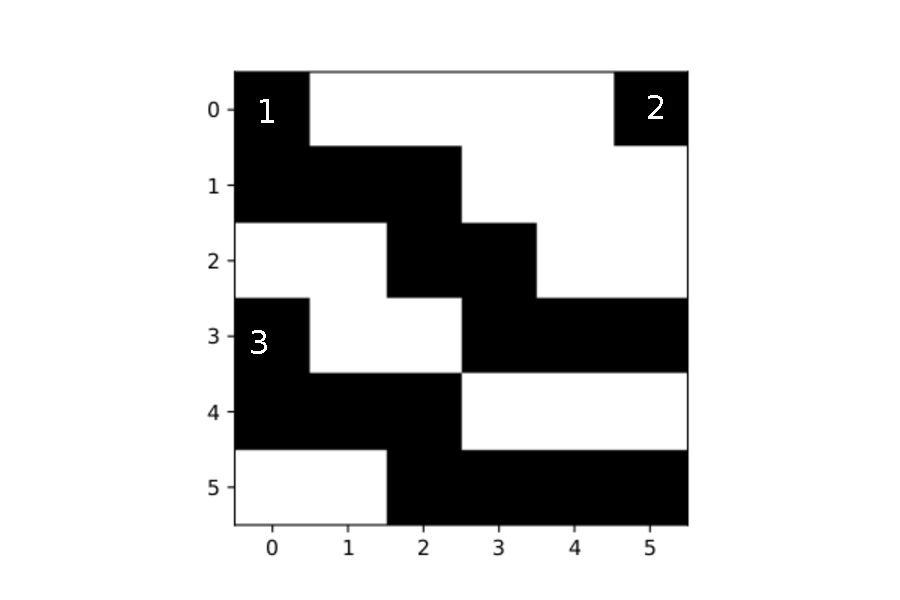
\includegraphics[scale=0.6]{diagonalperc1.pdf}
	\caption{Beispiel eines diagonal perkolierenden Clusters}
\end{figure}
\vspace{0,5cm}
\noindent Neben den in §\ref{gerichtet} beschriebenen gerichtet perkolierenden Clustern existieren noch Custer die diagonal über die periodischen Randbedingungen perkolieren. Ein Beispiel ist in Abbildung 4 zu sehen, aus dem ersten Cluster gelangt man über periodische randbedngungen in den dritten Cluster, geht man aus der Position 5,5 nach unten gelangt man in den dritten Cluster in der oberen rechten Ecke, mit einem Schritt nach rechts ist man wieder in Cluster 1.
\\
\noindent Das Finden dieser Cluster stellt sich als schwieriger heraus, als das Finden der gerichtet perkolierenden Cluster, da man nicht einfach nur die Labels über die Periodischen Randbedinungen verlinken darf wie das nachfolgende Beispiel zeigt.
\begin{figure}[h!]
	\centering
	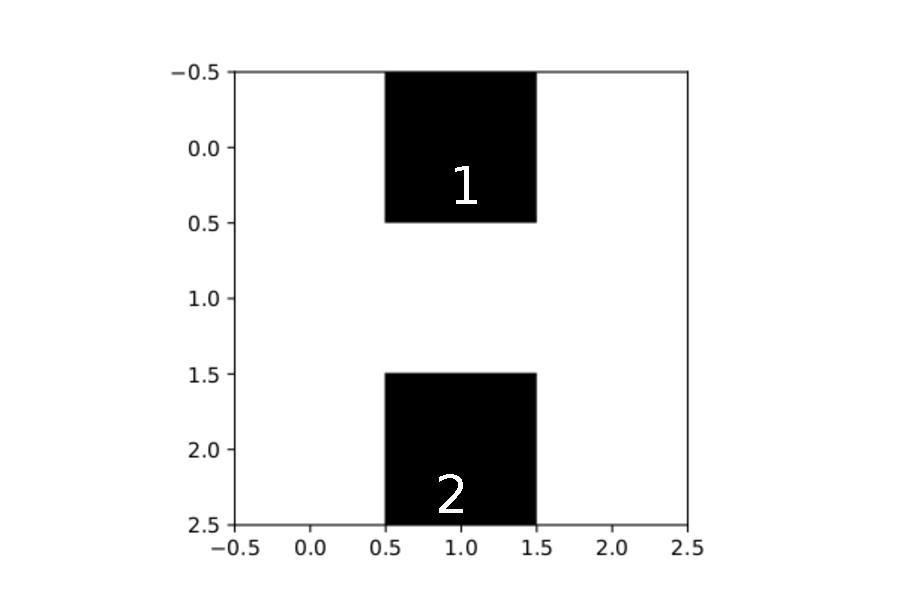
\includegraphics[scale=0.6]{noperc1.pdf}
	\caption{Es existiert offensichtlich kein perkolierender Cluster.}
\end{figure}

\vspace{0.5cm}
\noindent Würde man einfach das Labeln über periodische Randbedingung machen, würden beide Blöcke entsprechend Label 1 erhalten und nach dem Kriterium aus §1.2.2 hätte man einen perkolierenden Cluster gefunden. Dies ist ganz offensichtlich falsch, da es sich um einen Cluster endlicher Größe handelt.
\\
\noindent Der (scheinbar) korrekte Algorithmus den perkolierenden Cluster zu finden ist es, Cluster die sich über periodische Randbedinungen Berühren in einer Verlinkungsliste zu Speichern, zu den Labels muss die Richtung gespeichert werden. Man wählt die Konvention: links entspricht $(-1,0)$ rechts $(+1,0)$ unten $(0,-1)$ und oben entsprechend $(0,+1)$. Zu dem 'Weg' in der Verlinkungsliste muss die Summe der Richtungen gebildet werden, ist diese ungleich $(0,0)$ so perkolieren die Cluster die verlinkt sind. Man muss (rekursiv) eine Suchfunktion implementieren die alle zu einem gegebenen Label verlinkten Labels sucht. Auf alle Verlinkten Labels wird erneut die Suchfunktion angewendet, und so weiter, wird das Ausgangslabel gefunden so müssen die Richtungen addiert werden und mit $(0,0)$ verglichen werden.
\\
\noindent Am Beispiel der in Abbildung 4 gezeigten Matrix bedeuted die $1 \rightarrow 3$ hat Richtung $(+1,0)$, $3 \rightarrow 2$ bedeutet Richtung $(0,-1)$ und $2 \rightarrow 1$ wieder $(+1,0)$. Insgesamt hat dieser Weg also die Richtung $(+2,-1) \neq (0,0)$ und wird von dem Algorithmus gefunden.
\\
\noindent Im Gegensatz dazu zeigt die nächste Abbildung eine Matrix, mit einem $(0,0)$ Loop, man "läuft im Kreis", ohne das wirklich eine Box durchschritten wird. Diese Matrix wird auch nicht als perkolierend gefunden, eignet sich aber sehr gut zum debuggen.

\begin{figure}[h!]
	\centering
	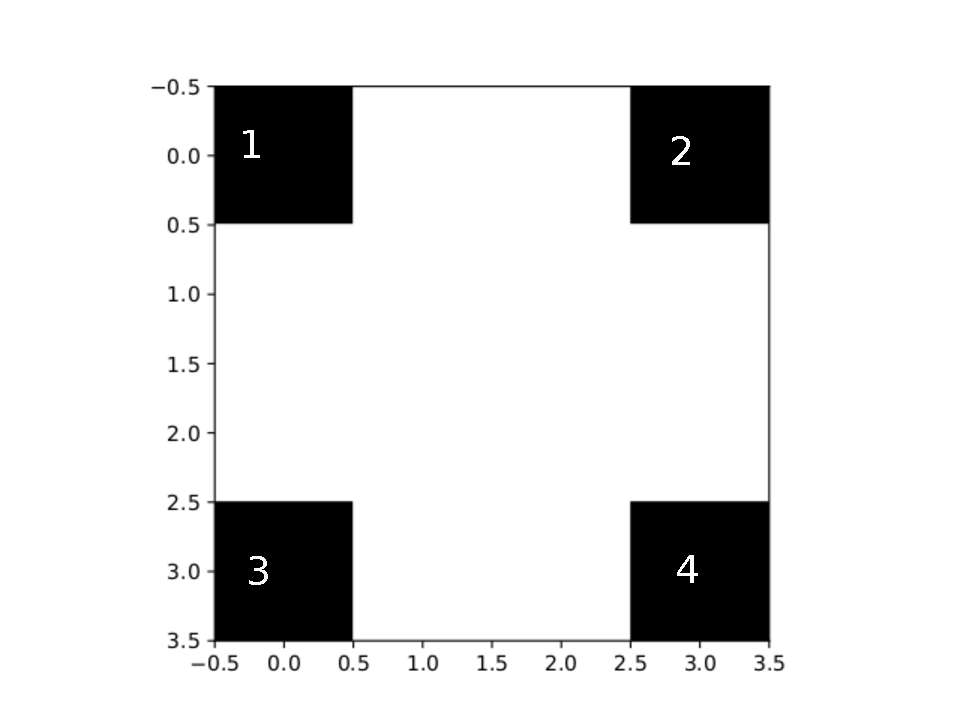
\includegraphics[scale=0.6]{noperc2.pdf}
	\caption{Es existiert offensichtlich kein perkolierender Cluster.}
\end{figure}

\noindent Das einzige Problem ist, dass dieser Algorithmus schlecht mit der Boxgröße skaliert, das die Anzahl der Labels quadratisch mit der Boxgröße skaliert und die Zahl der Knoten nochmals quadratisch mit der Boxgröße. Der Algorithmus skaliert also ungefähr mit $L^4$, wobei $L$ die Boxlänge bezeichnet. Unten sieht man den oben beschriebenen Teil zur Suche diagonal perkolierender Cluster als python Code, welcher auch in den nachfolgenden Simulationen genutzt worden ist.

\begin{figure}[h!]
	\centering
	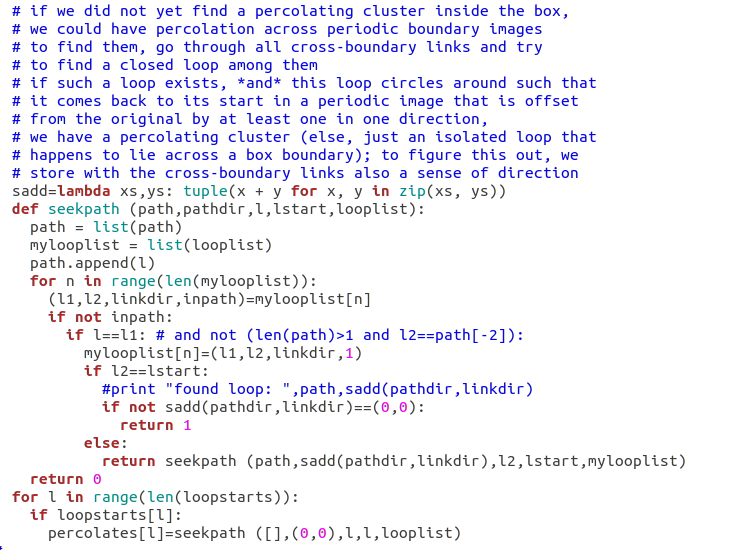
\includegraphics[scale=0.9]{diagcode.png}
	\caption{Python-Code zur Suche diagonal perkolierender Cluster.}
\end{figure}

\clearpage

\section{Random-Walk in ungeordneten Medien}

\subsection{"Normeler"\ Random-Walk}
Der (diskrete) Random-Walk auf dem freien Quadratgitter mit Hüpfwahrscheinlichkeit $\frac{1}{d}$ auf jeden der $d$ nächsten Nachbarn, wobei $d$ die Dimension des Gitter bezeichnet, unterliegt bekanntlich normaler Diffusion. Das heißt, dass das mittlere quadratische Verschiebung (engl. mean squared displacement), welches im weiteren mit $msd$ abgekürzt wird, linear mit der Anzahl an Schritten anwächst. Im kontinuierlichen Fall gilt die bekannte Formel:
\begin{align*}
msd(t)\equiv \langle \delta r^2 (t) \rangle =2dDt\ ,
\end{align*}
wobei (wie oben) $d$ die Dimension und $D$ der Diffusionskoeffizient sind, und hier gilt $D=1$.

\subsection{Random-Walk auf dem Perkolationsgitter}
Das Perkolationsgitter bei dem nur ein zufälliger Bruchteil der Gitterplätze begehbar sind und die anderen geblockt sind ist ein besonders einfaches Modell für ein ungeordnetes Medium. Eine spannende Frage - die in den 70er und 80er Jahren des vergangenen Jahrhunderts durch eine Vielzahl von Computersimulationen geklärt wurde - ist, wie sich ein Random-Walker auf so einem unregelmäßigen Perkolationgitter für verschiedene $p$ ($=$ Wahrscheinlichkeit das ein Gitterplatz begehbar ist) verhält. Speziell geht man, motiviert durch die fraktale Struktur der Cluster, von einem Potenzgesetz:
\begin{align*}
msd(t) \sim t^{2 \nu},\ \ \nu=1/d_w
\end{align*} 
aus, wobei $\nu$ als Diffusionsexponent bezeichnet wird und $d_w$ als 'walk dimension'. Der im Feld der weichen Materie bekannte französische Physiker Pierre-Gilles de Gennes nannte diese Fragestellung 1976 die 'Ameise im Labyrinth'.\cite{Stauffer} 
\\ 
\noindent Zuerst muss man die Hüpfwahrscheinlichkeiten festlegen, also ob $\frac{1}{f.n.N.}$ ($f.n.N.$ für freie nächste Nachbarn) oder wie bei dem freien Random-Walk $\frac{1}{d}$ und Züge auf ein geblocktes Feld werden zurückgesetzt. Für lange Zeiten sind beide Variaten äquivalent ('blind' vs 'myopic' ants)\cite{Havlin}.
\\
Nun überlegt man sich leicht die beiden Extremfälle $p$ nahe $1$ und $p$ nahe $0$. Im ersten Fall ($p \approx 1$) erwartet man sofort, dass $\nu \rightarrow1/2$, da es kaum 'Hindernisse' gibt und der Random-Walk nahezu ungestört laufen kann. Anders herum, bei $p$ nahe $0$ erwartet man, dass es keine perkolierenden Cluster gibt, somit ist der Random-Walker 'eingesperrt' in sogenannte 'Taschen', damit das $msd$ beschränkt und somit $\nu \rightarrow 0$ für lange Zeiten. Besonders spannend ist dieses Problem also in der Nähe der Perkolationsschwelle $p=p_c$, hier findet sich ein Diffusionskoeffizient, der weder $1/2$ noch $0$ ist. Gefen, Aharony und Alexander nannten diesen Effekt, dass das $msd$ weder normal (linear, $\nu = 1/2$) mit $t$ anwächst noch beschränkt ist, sondern für lange Zeiten asymptotisch einem Potenzgesetz mit $\nu \neq 1/2$ folgt, 'anormale Diffusion'.\cite{PhysRevLett.50.77} Diese anormale Diffusion wird, im Falle des unendlich großen Gitters, nur für $p=p_c$ gefunden, den für $p<p_c$ existiert kein perkolierender cluster, das $msd$ ist also beschränkt. Ist $p > p_c$ so gilt für $t \rightarrow \infty $ immer $msd \sim t$, aber es gibt ein 'Fenster' mit $msd \sim t^{2\nu}$, wobei $\nu < 1/2$ ist (siehe auch \cite{Kammerer_2008} für ein schematisches Bild mit 'Fenster').

\subsection{Chemische Distanz}
Prinzipiell muss man um über $msd$'s zu sprechen zuerst ine Metrik festlegen um Abstände zu messen. Meist wird (wie hier auch geschehen) ohne Erwähnung einfach die Euklidische Metrik genutzt. Im Fall von ungeordneten Medien und besonders von perkolierenden Clustern kann auch die sogenannte 'chemische Distanz/Metrik' genutzt werden, welche wie folgt definiert ist:
'Die chemische Distanz zwischen Gitterplatz $a$ und Gitterplatz $b$ bezeichnet die minimale Anzahl Schritte um (auf erlaubtem Wege) von $a$ nach $b$ zu kommen.' 
\\
\noindent Diese chemische Distanz kann auf dem perkolierenden Cluster offenbar stark von der Euklidischen Distanz abweichen, da Hindernisse 'gerade' Wege blockieren können und 'Umwege' erfordern.
 

\subsection{'all-cluster-' und 'percolating-cluster average'}

Es gibt im Allgemeinen zwei Varianten wie man $\nu_{pc}$ auffassen kann, man mittelt über zufällige Startpunkte auf dem zufällig geblockten Quadratgitter oder man mittelt über Startwerte die nur auf dem perkolierenden Cluster liegen ('all-cluster average' und \\ \noindent'percolating-cluster average'). Es ist zu erwarten, dass der Exponent bei dem 'all-cluster average' unter dem Exponenten des 'percolating-cluster average' liegt, da beim 'all-cluster average' auch in sogenannten Taschen gestartet wird in denen das $msd$ beschränkt ist. Die aktuell bekannten 'Literaturwerte' sind $d_w^{a.c.} \approx 3.036$ und $d_w^{p.c.} \approx 2.878$, woraus sich $\nu_{pc}^{a.c.} \approx 0.329$ und $\nu_{pc}^{p.c.} \approx 0.347$ ergeben.\footnote[4]{P. Grassberger, Phys. A 262, 251 (1999)} In dieser Spezialisierung wurde versucht diese Werte durch Monte-Carlo-Simulation (MC) zu reproduzieren. Es wurde eine Gitterlänge $L=1000$ verwendet und die Perkolationsschwelle als $p_c = 0.592\ 746$ angenommen. Es wurden zu beiden Mittelungsvarianten über $100$ Läufe auf je $100$ zufälligen Matrizen gemittelt, wobei nicht auf diagonale Perkolation getestet worden ist (aus Laufzeitgründen). Die Läufe waren je $10^6$ MC-Schritte lang und wurden auf einem ($10$er-) logarithmischen Grid gespeichert mit 48 Speicherstellen. 
\begin{figure}[h!]
	\centering
	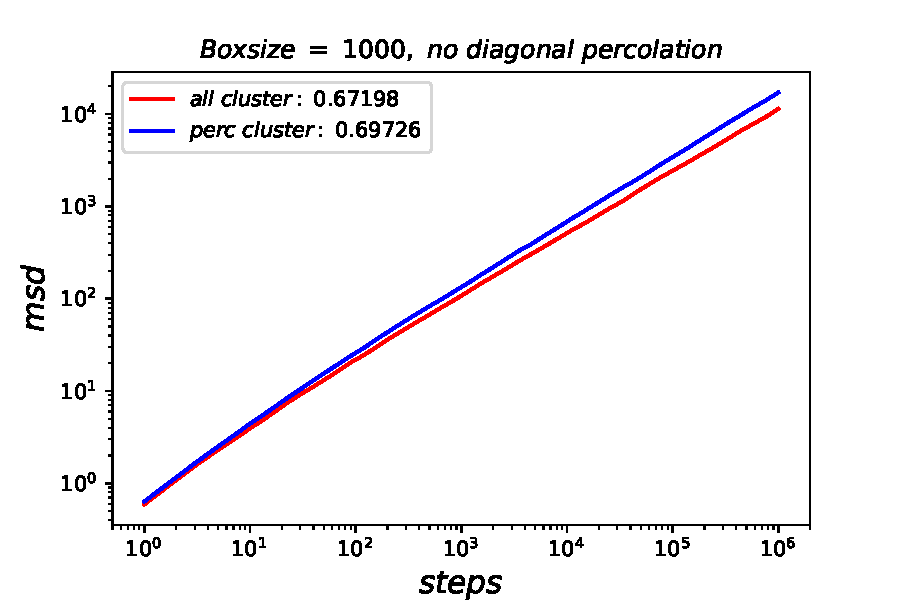
\includegraphics[scale=0.9]{acpcold1000.pdf}
	\caption{Ergebnisse meiner python3 MC-Simulation, der 'all-cluster average' ist in rot, der 'percolating-cluster average' in blau, es wurden keine diagonal perkolierenden Cluster in die Statistik aufgenommen.}
\end{figure}
\vspace{0,5cm}
\newpage
\noindent Die Exponenten wurden über einen $scipy.optimize.curve\_fit$ als $2\nu_{pc}^{a.c.} \approx 0.6712$ und $2\nu_{pc}^{a.c.} \approx0.6973$ bestimmt. Die Methode den Exponenten durch einen fit zu bestimmen hat sich als deutlich stabiler herausgestellt als das bestimmen der Ableitung durch eine 'central-difference' oder 'forward-difference' Methode, welche unter sehr hohen numerischen Fehler leiden, da zwei sehr große Zahlen von einander abgezogen werden, deren Differenz klein ist. Dieses Problem ist bekannt als 'catastrophic cancellation'. Nimmt man Werte die weiter auseinander liegen (also ein größeres $h$), so wird die Ableitung ebenfalls sehr ungenau, da der Fehler quadratisch ('central-difference') beziehungsweise linear ('forward-difference') in Abstand $h$ wächst. Ein lokaler Mittelwert hilft etwas,
die 'Zacken' in der numerischen Ableitung zu glätten, ist aber durch das logarithmische Grid mit Vorsicht zu genießen, da spätere Zeiten stärker gewichtet werden. Im nachfolgenden Plot ist die numerische Ableitung mit dem Fit-Parameter verglichen und ebenfalls die gefittete Kurve (in schwarz) an das 'all-cluster' mean-squared-displacement angelegt. Man erkennt, dass die numerische Ableitung, welche ähnlich zur 'central difference', aber auf einem logarithmischen Grid ist, und Fit übereinstimmen. Auf oben beschriebenes Glätten der Ableitung wurde verzichtet. 
\begin{figure}[h!]
	\centering
	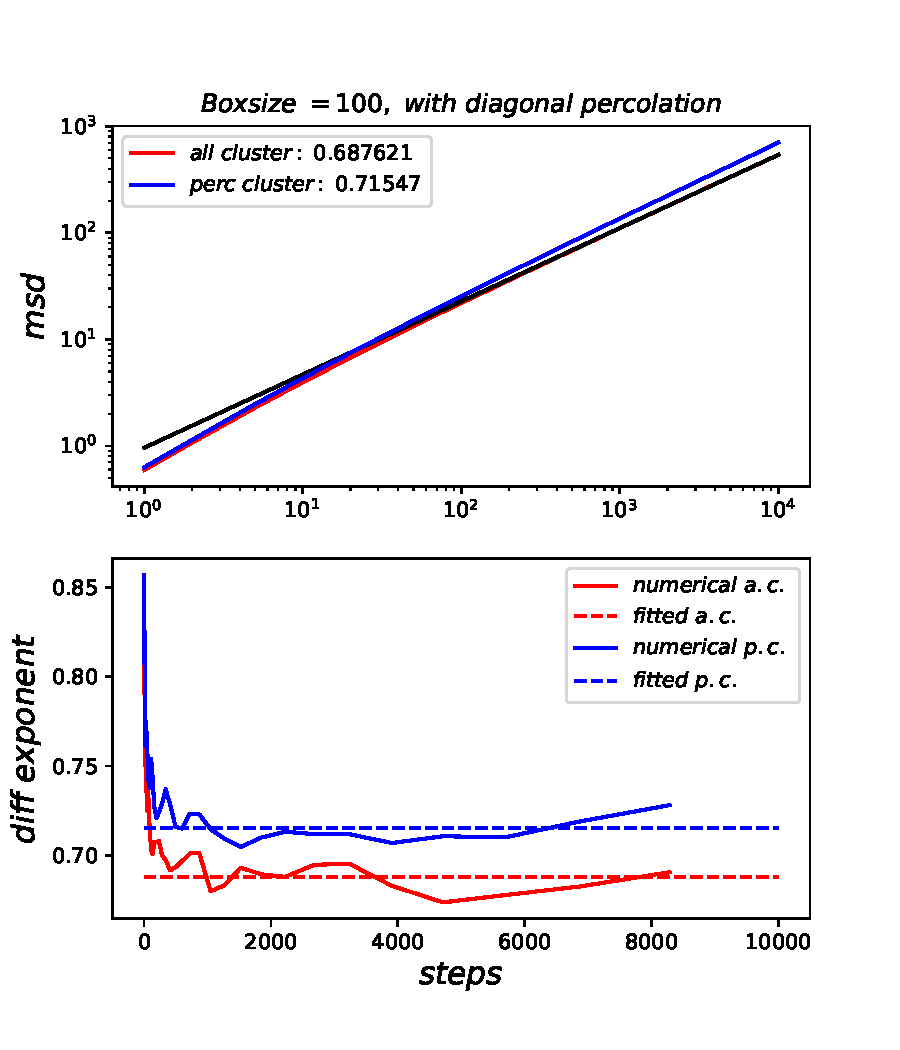
\includegraphics[scale=0.9]{newacpc100.pdf}
	\caption{Ergebnisse meiner python3 MC-Simulation, der 'all-cluster average' ist in rot, der 'percolating-cluster average' in blau, es wurden keine diagonal perkolierenden Cluster in die Statistik aufgenommen.}
\end{figure}
\newpage


\subsection{Vergleich der Statistik mit und ohne diagonale Perkolation}
\noindent In kleineren Simulationsboxen treten finite-size Effekte auf. Die Diffusionsexponenten sind weiter von den Literaturwerten für eine unendliche Box entfernt; dennoch sind (bei gleicher Boxgröße) wie nachfolgender Plot zeigt die Exponenten mit diagonal perkolierenden Clustern näher am Literaturwerten für eine unendliche Box. Es sind bei einer Boxgröße $L=100$ ca. $18,6\%$ der perkolierenden Cluster diagonal perkolierend. Größere Boxen sind aktuell durch zu hohe Laufzeit des Clustersuch-Algorithmus nicht (im Rahmen einer Masterarbeit, bzw. deren Einarbeitung) realisierbar.
\begin{figure}[h!]
	\centering
	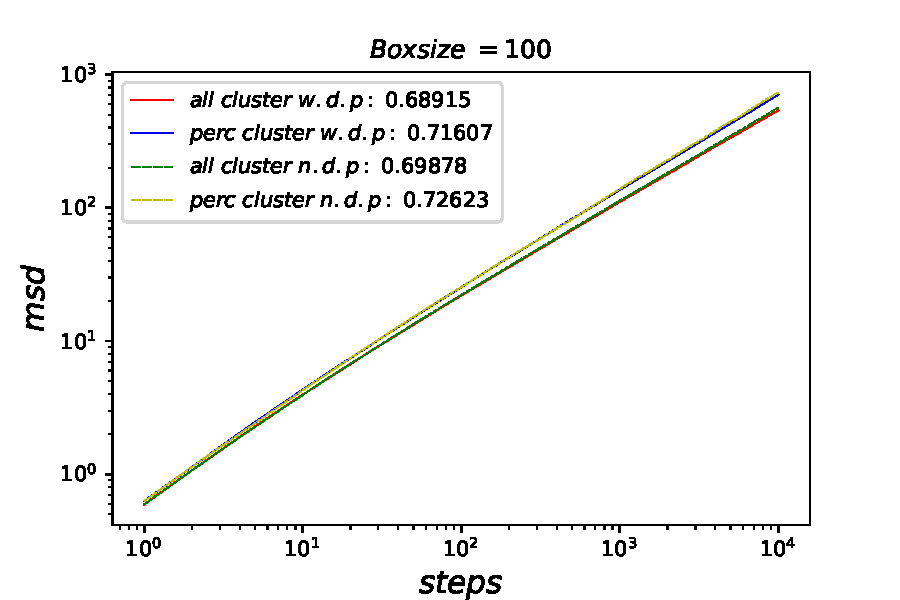
\includegraphics[scale=0.9]{both100.pdf}
	\caption{Vergleich von Statistik mit (w.d.p.) und ohne (n.d.p.) diagonal perkolierende Cluster. Gesamplet über 1000 Läufe auf je 500 Matrizen.}
\end{figure}

\noindent Man sieht vorallem an den Werten, das der Literaturwert von $2\nu_{pc}^{p.c.} \approx 0.694$ nun unterschätzt wird (bezogen auf den 'percolating-cluster average'). Zudem ist der Wert bei der Box mit Länge $L=1000$ ohne diagonal perkolierende Cluster näher am Literaturwert. Man sollte also lieber auf das finden der diagonal perkolierenden Cluster verzichten und größere Boxen wählen, denn der 'finite-size' Fehler scheint größer, als der Fehler, den das Auslassen der diagonal perkolierenden Cluster verursacht.
\subsection{Random-Walk auf diagonal perkolierenden Clustern}
Um den Einfluss der diagonal perkolierenden Cluster besser zu verstehen habe ich eine Simulation von 1000 Läufen auf je 500 diagonal perkolierenden Clustern angefertigt ('percolating-cluster average'). Die Boxgröße beträgt $L=100$. Es wurde $\nu_{pc}^{p.c.} \approx 0.681$ gefunden, dieser Wert unterschreitet den Literaturwert von $\nu_{pc}^{p.c.} \approx 0.694$. Dies ist leicht einzusehen, den diagonale Läufe haben ein geringeres $msd$, da ein Schritt nach (z.B.) rechts gefolgt von einem Schritt nach (z.B.) oben ein $msd$ von $2$ ergibt wohingegen zwei Schritte in eine Richtung ein $msd$ von $4$ ergeben. Die diagonal perkolierenden Cluster führen also auch dazu, dass das $msd$ geringer wird, so lässt sich erklären, das auch bei der Simulation der $L=1000$ Box in §2.3 beide Exponenten überschätzt werden.

\begin{figure}[h!]
	\centering
	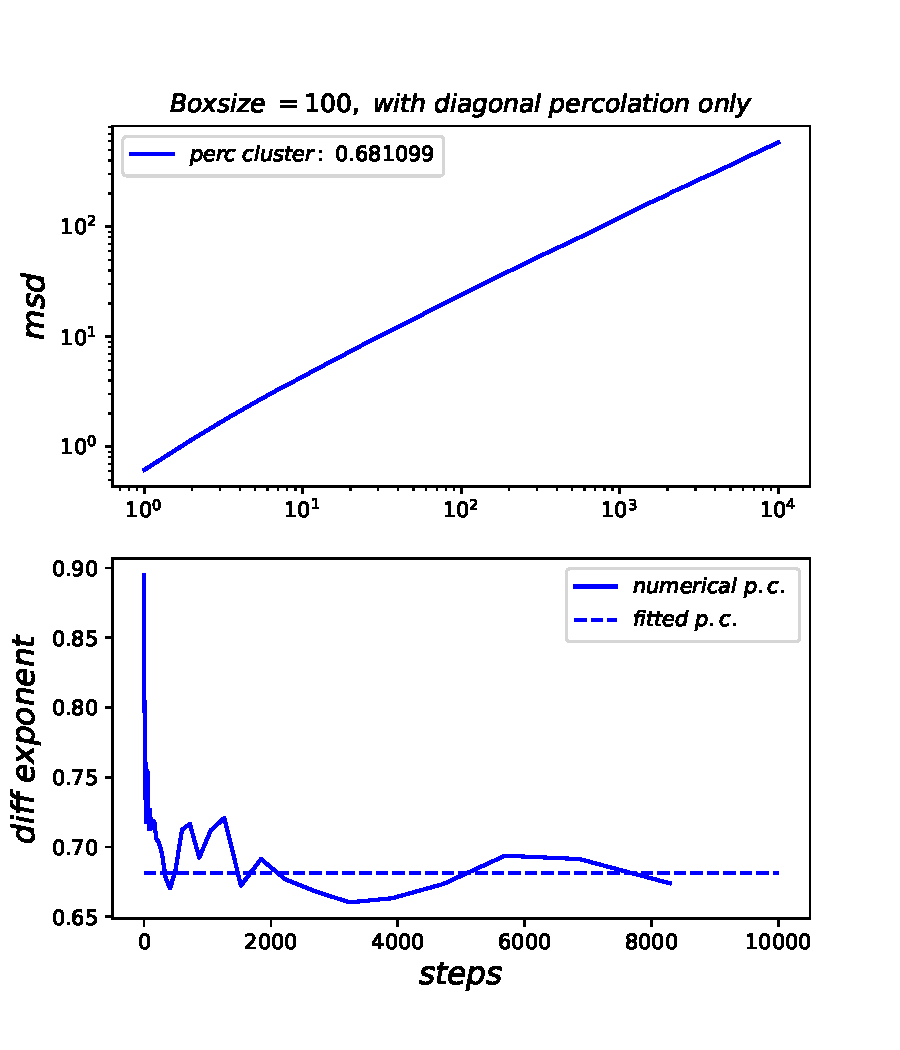
\includegraphics[scale=0.9]{diagpc100.pdf}
	\caption{Vergleich von Statistik mit und ohne diagonal perkolierende Cluster. Gesamplet über 1000 Läufe auf je 500 Matrizen.}
\end{figure}


\newpage


\subsection{Self-Avoiding Walk auf dem Perkolationsgitter}
Self-Avoiding Walks (kurz: SAW), also Random-Walks die niemals zu einem zuvor besuchten Gitterplatz zurückkehren sind ein Standardthema in der Physik der weichen Materie, da sie ein Modell für Polymerketten geben und meist auch eins der ersten Beispiele für einen nicht-markovschen stochastischen Prozesss. Der Exponent $\nu^{SAW}$ des $msd$ beim SAW ist daher von besonderem Interesse, da er eine Verbingung zwischen mittlerer Größe eines Polymers und der Anzahl der Kettenglieder schafft:
\begin{align*}
\tilde R \equiv \sqrt{\langle R^2 \rangle} \sim N^{\nu^{SAW}},
\end{align*} 
wobei $\tilde R$ der Durchmesser des Polymers ist.
\\
Nun lässt sich auch leicht die Frage formulieren wie sich ein SAW auf dem Perkolationsgitter ausbreitet. Der normale Random-Walk ist langsamer geworden, genauer: $\nu_{pc} \equiv \nu_{pc}^{p.c.} < 1/2$, im Gegensatz dazu wird der SAW auf dem Perkolationsgitter schneller. In anderen Computersimulationen wurde $\nu^{pcSAW} \approx 0.78$ gefunden wohingegen $\nu^{SAW}=3/4=0.75$ ist\footnote[5]{V. Blavatska und W. Janke, Europhy. Lett. 82, 6606 (2008)}$^,$\footnote[6]{N. Fricke und W. Janke, Europhys. Lett. 99, 56005 (2012)}. Die Nachstehende Graphik zeigt, das auch endliche SAW sich auf dem p
Perkolationscluster schneller ausbreiten als auf dem freien Gitter\footnote[7]{Lee, Nakanishi und Kim, Phys. Rev. B 39, 13 (1989)} Der SAW ist ein wichtiger Vergleich zu dem 'aktiven' Random-Walk.
\begin{figure}[h!]
	\centering
	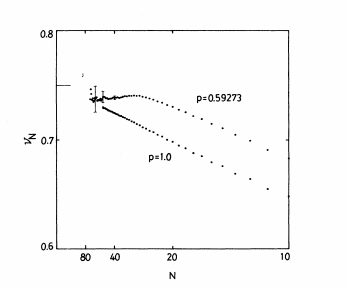
\includegraphics[scale=1.2]{saw.png}
	\caption{Ergebnisse einer MC-Simulation von Lee, Nakanishi und Kim. $N$ bezeichnet die Länge des SAW's.}
\end{figure}

\subsection{'Aktiver' Random-Walk auf dem Perkolationsgitter}
Es wird nun eine Variante des Random-Walk betrachtet, welche zuvor noch nicht besuchte Plätze bevorzugt. Diese Variante eines Random-Walks kann man zum Beispiel für die Modellierung von Chemotaxis von Bakterien verwenden. Das Modell sieht wie folgt aus: man generiert zuerst das Perkolationsgitter, danach werden begehbare Gitterplätze mit 'Nahrung' belegt, welche vom Random-Walker bei dem Besuch des jeweiligen Gitterplatzes vollständig 'gegessen' wird. Der Random-Walk erinnert also an 'Pacman' der durch ein Labyrinth (den perkolierenden Cluster) nach Nahrung absucht.
\begin{figure}[h!]
	\centering
	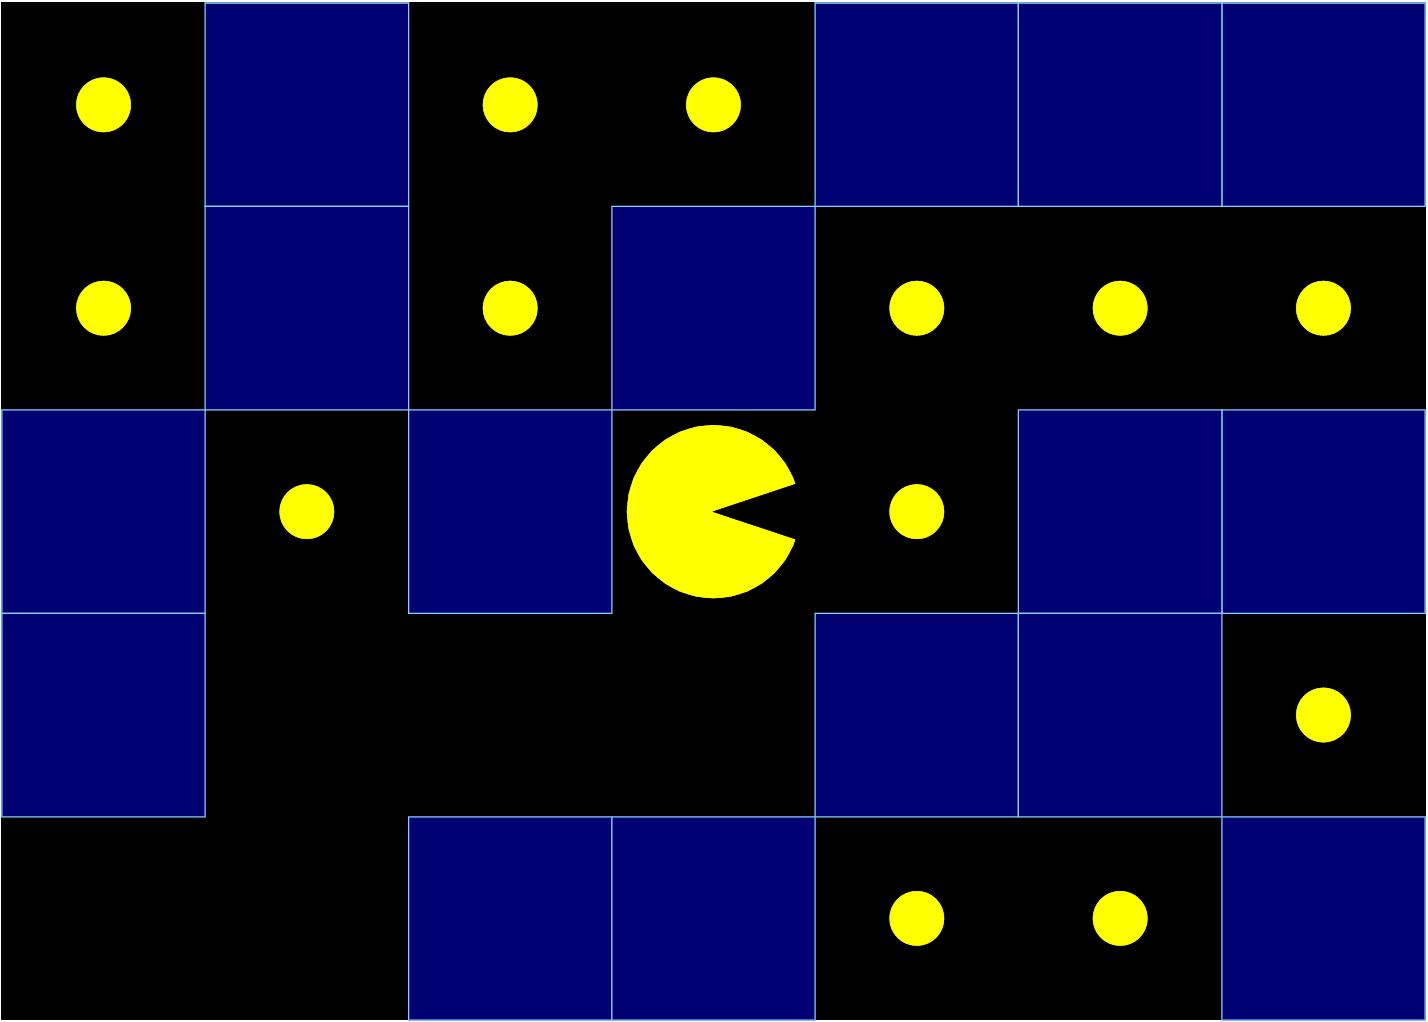
\includegraphics[scale=0.25]{pacman.png}
	\caption{Veranschaulichung des Modells, blaue Quadrate sind geblockte Gitterplätze, kleine gelbe Kreise sind Nahrung und 'Pacman' ist der Random-Walker.$^8$}
\end{figure}
\newpage


\noindent Die Wahrscheinlichkeiten für den nächsten Zug werden gemäß:
\begin{align}
p_{j \leftarrow i} = \frac{exp({F_j})}{\sum_j exp({F_j})}
\end{align}
berechnet, wobei $F_j$ die Menge der Nahrung an Gitterplatz $j$ ist, also $F$ falls Gitterplatz $j$ noch nicht besucht worden ist und $0$ falls Gitterplatz $j$ zuvor bereits besucht wurde, $i$ ist dabei der Gitterplatz auf dem der Random-Walker aktuell ist. Dieses Modell scheint, insbesondere für $F \rightarrow \infty$, zuerst dem SAW sehr ähnlich zu sein, welcher auf dem Percolationsgitter schneller wird. Monte-Carlo-Simulation dieses 'aktiven' Random-Walkers auf dem Perkolationsgitter zeigt, das der Exponent kleiner ist, als der des normalen Random-Walkers auf dem Perkolationsgitter. Die Nachstehende Abbildung zeigt Ergebnisse einer Monte-Carlo-Simulation mit je $100$ Walks auf $100$ Perkolationsgittern (Matrizen), wobei nicht auf diagonale perkolation getestet worden ist, mit einer Größe von $1000 \times 1000$. Die Nahrung wird in meiner Simulation immer aus der Originalmatrix gelöscht und somit auch aus allen Kopien, welche durch die periodischen Randbedinungen entstehen, diese Methode ist zwar nicht ganz Korrekt (Quelle für finite-size-Effekte), führt aber zu keinem sichtbaren Fehler, solange die Wurzel aus dem $msd$ kleiner als die Boxgröße ist. Der Vorteil ist, dass diese Methode schneller ist und weniger Speicher benötigt. Die Perkolationsschwelle wurde wie zuvor als $p_c=0.592746$ angenommen.
\begin{figure}[h!]
	\centering
	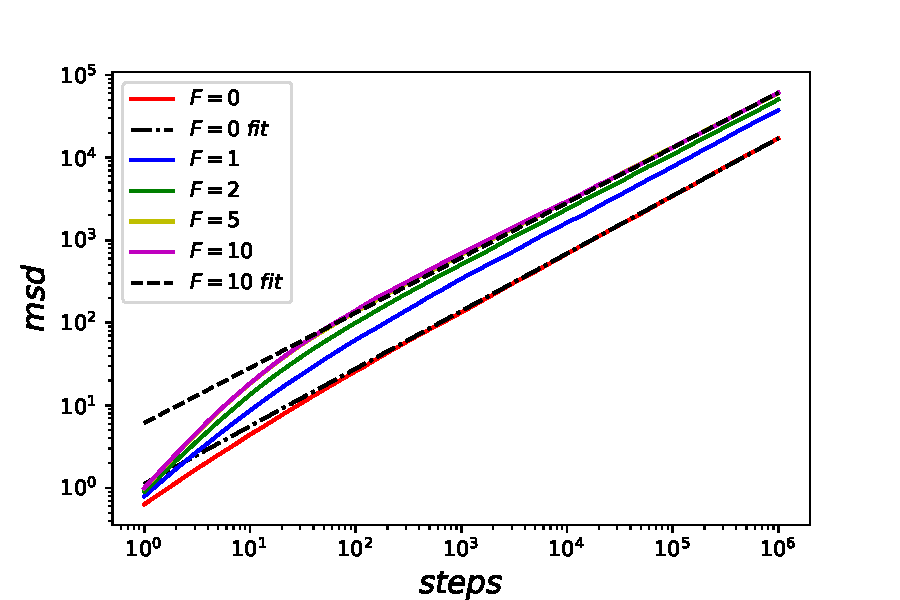
\includegraphics[scale=0.9]{food.pdf}
	\caption{Ergebnisse meiner python3 MC-Simulation des 'aktiven' Random-Walkers auf perkolierendem Cluster ohne diagonale Perkolation. Die gestrichelten Linien sind die mit scipy bestimmten langzeit power-laws.}
\end{figure}
\newpage

\noindent Es lässt sich erkennen, dass mit steigendem $F$ der Diffusionsexponent $\nu$, also die (halbe) Steigung der Kurve abnimmt, entgegen der naiven Annahme, das je größer $F$ ist, desto ähnlicher wird dieses Modell dem SAW.
Es wurden die folgenden Diffusionskoeffizienten gefunden:

\begin{tabular}[h]{l|c}
	F & $2\nu(F)$\\
	\hline
	0 & 0.697\\
	1 & 0.682\\
	2 & 0.664\\
	5 & 0.655\\
	10 & 0.666\\
\end{tabular}

\noindent Das gleiche Verhalten wurde auch bei einer kleineren Box von $L=100$ gefunden. Es wurde über 1000 Läufe auf je 100 Perkolationsgittern (inklusive diagonaler Perkolation) gemittelt.
\begin{figure}[h!]
	\centering
	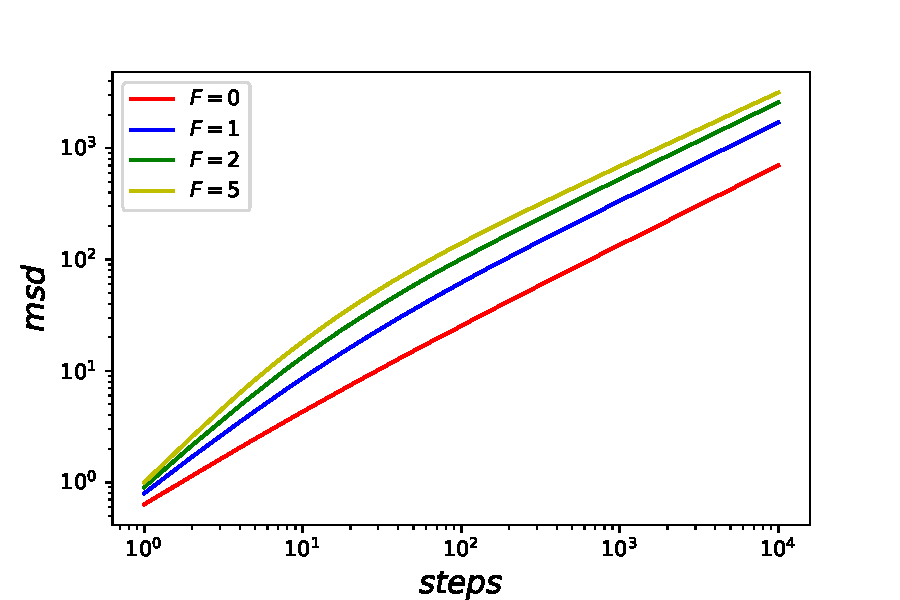
\includegraphics[scale=0.9]{newfood.pdf}
	\caption{Ergebnisse meiner python3 MC-Simulation des 'aktiven' Random-Walkers auf perkolierendem Cluster mit diagonaler Perkolation.}
\end{figure}
\newpage 
\noindent Erneut wurde die Nahrung die 'Pacman gegessen hat' aus der originalen Matrix und somit auch aus allen Kopien die durch die periodischen Randbedingungen entstehen gelöscht. Die Wurzel aus dem $msd$ ist erneut kleiner als die Boxlänge $L=100$.\\
\noindent Dieses Modell zeigt auch sehr schön den Unterschied zwischen fraktaler und Random-Walk Dimension, da das Perkolationsgitter (also die fraktale Dimension $\approx 1.7\ -\ 1.8$)\footnote[9]{R F Voss, J. Phys. A, 17, 7 (1984)} unabhängig von $F$ ist, die Random-Walk Dimension (also $1/\nu$) aber nicht.
\newpage
\noindent Monte-Carlo-Simulationen mit einer Boxgröße von $L=25000$ und bis zu $10^6$ Walks auf bis zu $100\ 000$ Matrizen zeigen das gleiche Verhalten. In diesen Simulationen\footnote[8]{T. Schilling und T. Voigtmann, J. Chem. Phys. 147, 214905 (2017)} wurden die bereits besuchten Gitterplätze korrekt mit einem 'hash-table' nachgehalten. Die Ergebnisse dieser MC-Simulationen befinden sich in der nachfolgenden Abbildung.

\begin{figure}[h!]
	\centering
	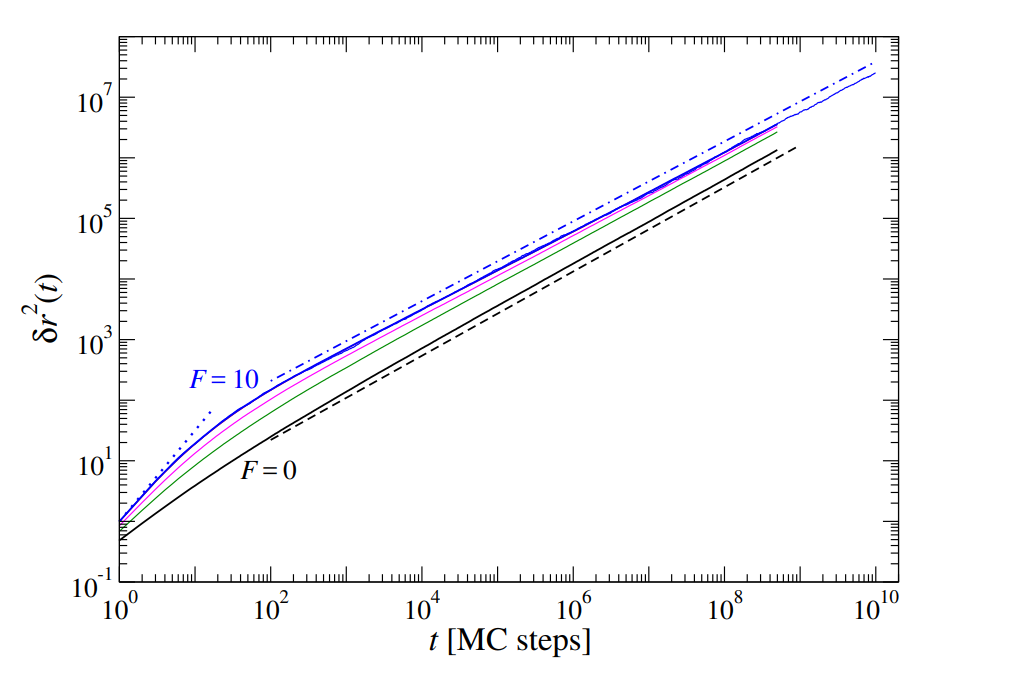
\includegraphics[scale=0.5]{food_thomas.png}
	\caption{Die blau gepunktete Linie zeigt die power-law des SAW ($\nu^{SAW}=3/4$), die blau gepunktet/gestrichelte Linie eine power-law zum Exponenten $\nu = 0.33$.}
\end{figure}

\chapter{Viele Random-Walker auf dem freien Cluster mit Nahrung (2D)}
\section{Interaktion der Random-Walker}
Die einzelnen Random-Walker haben keine direkte Interaktion untereinander, es ist also insbesondere auch möglich, dass zwei (oder mehrere) Random-Walker auf der gleichen Position im Gitter sitzen. Der einzige Wechselwirkungseffekt der bei diesem Modell vorliegt ist, dass die Walker sich gegenseitig 'Nahrung wegessen' und somit die Umgebung eines anderen Walkers verändern und damit auch die Wahrscheinlichkeiten wohin der nächste Schritt ausgeführt wird. Es wurden zwei Zugversionen getestet, einmal ziehen alle Random-Walker zur selben Zeit und alternativ ziehen die Random-Walker sukzessive, also zuerst Random-Walker 1, gefolgt von Random-Walker 2 und so weiter. \\
\noindent Die Wahrscheinlichkeiten, wohin ein Random-Walker zieht werden wie in [XX] gemäß:
\begin{align}
p_{j \leftarrow i} = \frac{exp({F_j})}{\sum_j exp({F_j})}
\label{Wkeiten}
\end{align}
berechnet, wobei $F_j$ die Menge der Nahrung an Gitterplatz $j$ ist.

\section{Klassischer gegen sukzessiver Algorithmus}
Wie im vorigen Kapitel angekündigt, werden zwei verschiedene Zugvarianten der hungrigen Walker gegeneinander verglichen. Dies dient dazu um zu prüfen ob der im nachfolgenden beschriebene Effekt kein Artefakt der Zugversion ist.
\\
\noindent Es wird falls nicht anders angegeben über 1000 Läufe gemittelt. Da es 1000 Walker gibt mittelt man so über $10^6$ einzelne $msd$. Eine deutlich 'bessere' Statistik ist aus Gründer der Laufzeit beziehungsweise der Rechnerkapazitäten nicht möglich. Zudem erscheint die Anzahl an Samples ausreichend.
\\
\noindent Es stellt sich heraus, dass man ein nahezu identisches Ergebnis aus den beiden Monte-Carlo-Simulationen erhält. Der im nächsten Kapitel beschriebene Effekt ist daher stabil gegenüber der verwendeten Zugversion.
\\
\noindent Es wird im weiteren daher die zuerst vorgeschlagene Zugversion verwendet.

\begin{figure}[h!]
	\centering
	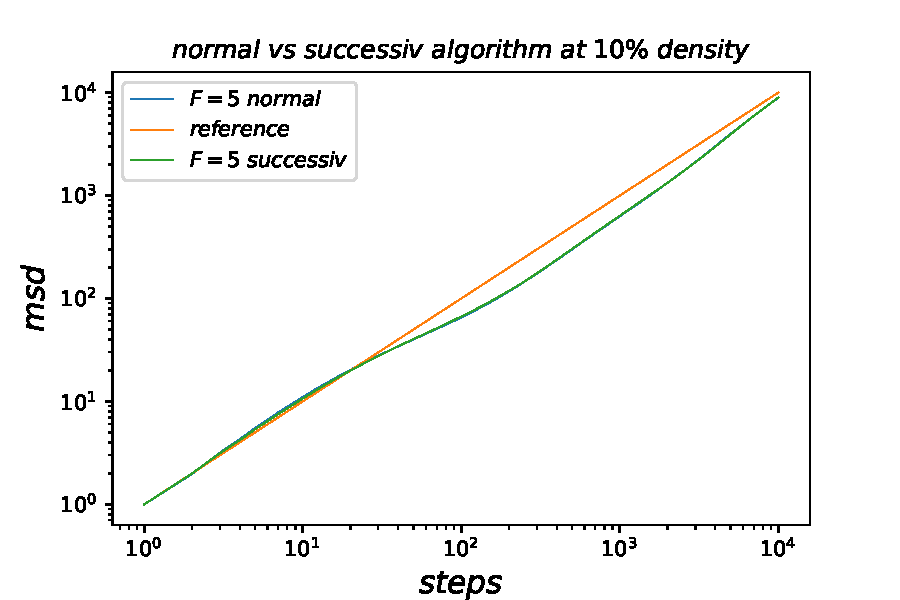
\includegraphics[scale=0.9]{suc.pdf}
	\caption{Monte-Carlo Ergebnisse der beiden Zugversionen für das $msd$ von $1000$ Walkern auf einem (für $F\neq0$) mit Nahrung bestückten freien $100\times 100$ Gitter (also einer Dichte von 10\%). Die Kurve 'reference' bezeichnet: $msd(t)=t$.}
\end{figure}

\newpage 

\section{Auftreten eines streng subdiffusiven Regimes}
Durch Monte-Carlo-Simulation wurde das $msd$ für ein $100 \times 100$ Gitter und $1000$ Random-Walkern ermittelt. Es lässt sich für $F=2$ und besonders für $F=5$ ein streng subdiffusives Regime erkennen, das heißt ein Bereich, in dem das $msd$ kleiner ist als das $msd$ des freien Random-Walks ohne Nahrung ($F=0$) und mit geringerem Diffsuionsexponenten steigt (also anormale Diffusion vorliegt). Beachte, das wenn nur ein Diffusionsexponent $\nu < 0.5$ vorliegt von (nicht streng) subdiffusiv gesprochen wird.\\
\noindent Zudem liegt zu Beginn des Prozess Superdiffusion vor, das heißt der Random-Walker ist 'schneller' als der freie Random-Walk ($msd(t)=t$).\\
\noindent Der superdiffusive Bereich ist zu erwarten und lässt sich leicht erklären. Zu Beginn sind die Walker im mittel noch mehrere Gitterplätze voneinander entfernt und sehen nur ihren eigenen Zug und meiden daher (je höher $F$ ist desto stärker) in die entgegengesetzte Richtung zurückzukehren, ähneln also dem SAW. \\
\noindent Der Großteil dieses Kapitels beschäftigt sich mit der Erklärung des streng subdiffusiven Bereichs, welcher zunächst sehr merkwürdig erscheint und im Gegensatz zum superdiffusiven Regime nicht (naiv) zu erwarten ist.
\\
\noindent Zur Simulation muss erneut bemerkt werden, das die Nahrung (nach Besuch eines Walkers) aus der 'originalen' Matrix und somit auch aus allen periodischen Kopien gelöscht wird. Die Walks sind dementsprechend auf die Länge der Boxgröße zu beschränken um starken finite size Effekten vorzubeugen. Es wird zudem über alle Walker gemittelt um das $msd$ zu berechnen.
\\
\noindent In den nachfolgenden Unterkapiteln wird (hauptsächlich) der $F=5$ Fall bei 10\% Dichte untersucht, um eine Erklärung für das streng subdiffusive Regime zu finden. 

\noindent Die nachfolgende Abbildung zeigt das oben diskutierte $msd$ von 1000 Walkern auf einem mit Nahrung bestückten freien $L=100$ Gitter. Im Fall $F=5$ ist deutlich zu sehen, wie rund die ersten 20 Schtritte superdiffusiv sind und danach in ein streng subdiffusives Regime gewechselt wird. Die $F=0$ Kurve kann als Referenz angesehen werden, da ohne Nahrung absolut keine Wechselwirkung mehr zwischen den einzelnen Walkern besteht, womit ein normaler zweidimensionaler Random-Walk ausgeführt wird.

\begin{figure}[h!]
	\centering
	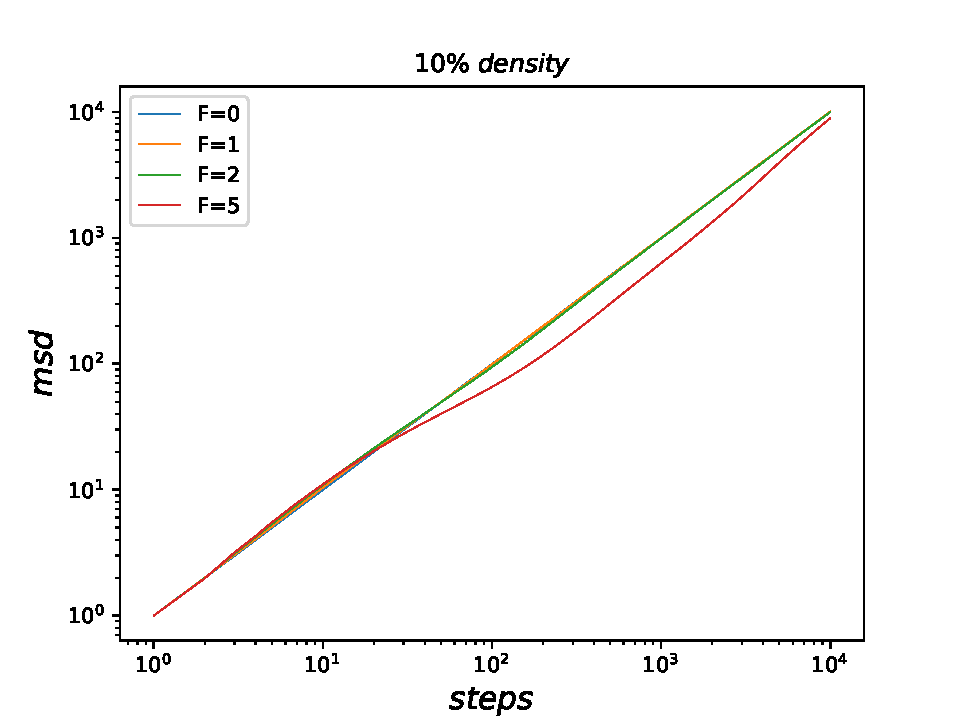
\includegraphics[scale=0.9]{mult_food.pdf}
	\caption{\label{vieleF}Monte-Carlo Ergebnisse für das $msd$ von $1000$ Walkern auf einem (für $F\neq0$) mit Nahrung bestückten freien $100\times 100$ Gitter (also einer Dichte von 10\%).}
\end{figure}

\newpage

\section{Fraktale Dimension der Nahrungsverteilung}
Der erste Versuch zur Erklärung des streng subdiffusiven Verhaltens der Random-Walker ist es, numerisch die fraktale Dimension der Nahrungsverteilung zu bestimmen, denn die Walker laufen mit sehr hoher Wahrscheinlichkeit auf mit Nahrung besetzten Feldern des Gitters (der Matrix) und somit hat die Struktur der Nahrungsverteilung einen Einfluss auf das $msd$ der Walker. Zudem wird der Anteil an vorhandener Nahrung gegen die MC-Schritte aufgetragen, die Nahrung wird auf den ersten Schritt normiert, das heißt es wird durch die mittlere Dichte der freien Felder zum Quadrat geteilt.
\subsection{Die Box-Counting-Methode}
Zur Bestimmung der fraktalen Dimension wird die sogenannte Box-Counting-Methode verwendet.\footnote[1]{\url{https://en.wikipedia.org/wiki/Box\_counting} 23.12.2019} 
\\
\noindent Es werden sukzessive Boxen von der Größe $l=2^n$ , $l=2^{n-1}$ , ... , $l=2$ gebildet und jeweils die Anzahl der mit Nahrung belegten Felder gezählt. Die fraktale Dimension ist dann der Exponent bzw. hier bei doppelt logarithmischer Auftragung der Vorfakter wie die Anzahl der Nahrungseinheiten mit der Boxgröße skalieren. Hier wurde eine leichte Veränderung des Codes von Nicolas P. Rougier verwendet\footnote[2]{\url{https://gist.github.com/rougier/e5eafc276a4e54f516ed5559df4242c0} 23.12.2019}.
\\
Genauere Details und mögliche Implementierung dieser Methode können dem nachfolgenden Python3 Code entnommen werden.
\begin{figure}[h!]
	\centering
	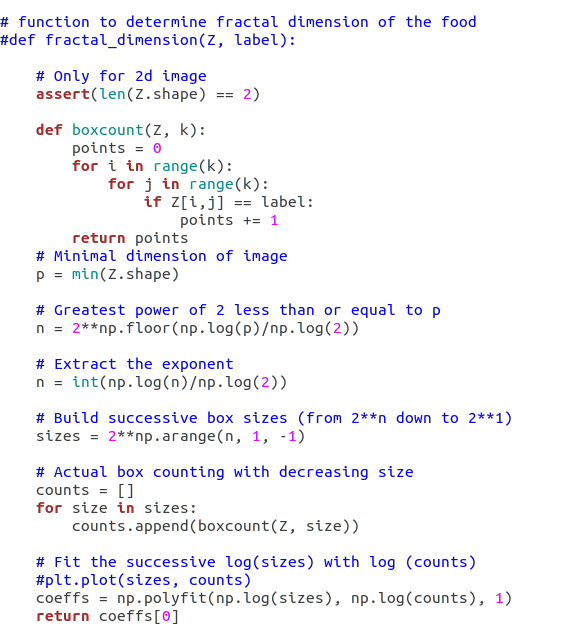
\includegraphics[scale=0.8]{fractal.png}
	\caption{Python3 Code für das Box-Counting zur Bestimmung der fraktalen Dimension der Nahrungsverteilung.}
\end{figure}

\newpage

\subsection{Ergebnisse der Box-Counting Analyse}
Die nachfolgende Abbildung zeigt die Ergebnisse der Box-Counting Analyse zur fraktalen Dimension der Nahrungsverteilung. Es ist (abseits von numerischen Schwankungen) keine Veränderung zu erkennen, da die Walker gleichmäßig in der Marix verteilt sind und somit auch die 'Fressspuren' gleichmäßig über die Box verteilt sind, das heißt in einer doppelt so großen Box ($ l \rightarrow 2l$) sind viermal so viele 'Fressspuren' und daher ist die numerisch bestimmte fraktale Dimension die gesamte Zeit ca. $2$.
\\
\noindent Die Box-Counting Methode wird also im weiteren Verlauf nicht mehr verwendet un wurde hier nur zur Vollständigkeit diskutiert. 

\begin{figure}[h!]
	\centering
	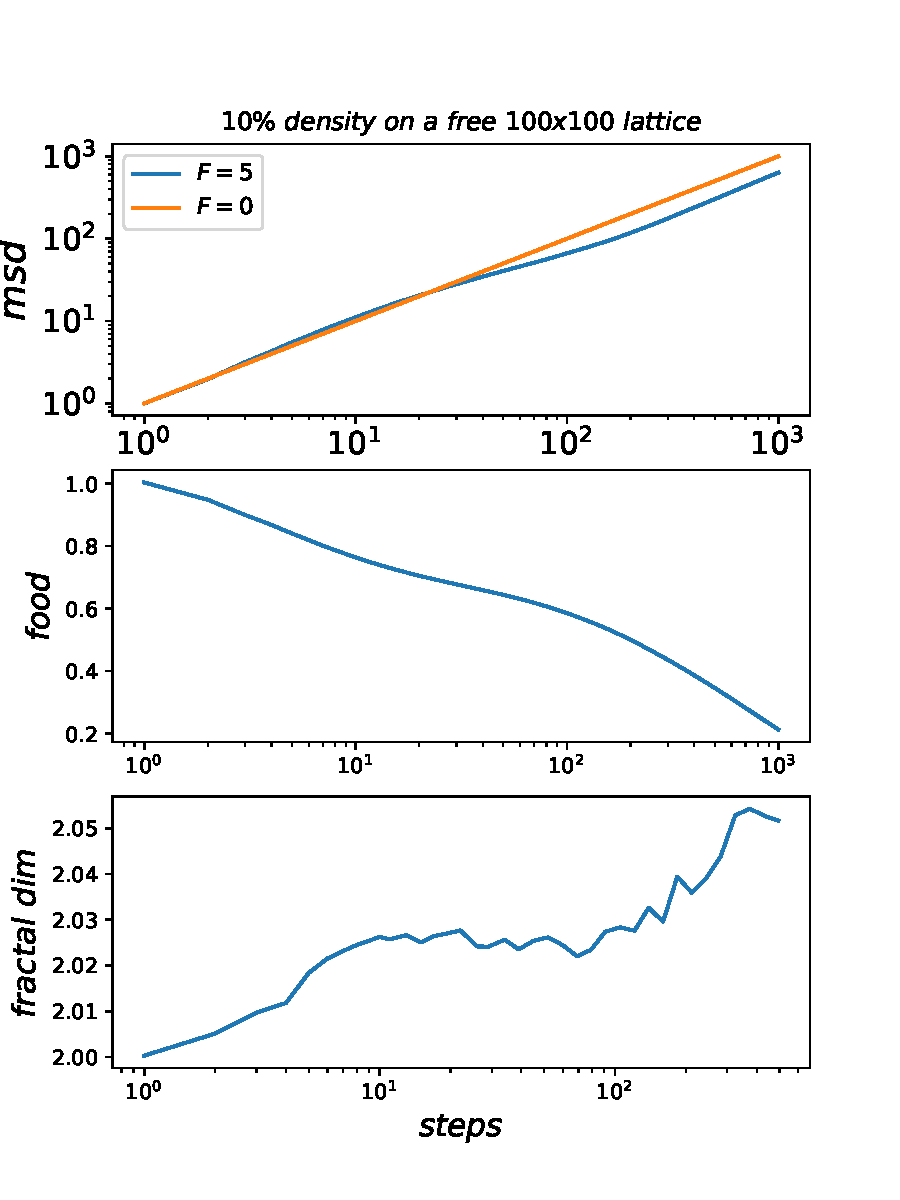
\includegraphics[scale=0.75]{10fractal.pdf}
	\caption{Ergebniss der Box-Counting Analyse bei 1000 Walkern auf dem $100\times 100$ Gitter mit $F=5$.}
\end{figure}

\newpage
\subsection{Nahrungsvorrat}
\noindent Man sieht ebenfalls in obiger Abbildung, das während des Wechsels von superdiffusiv zu streng subdiffusiv weniger Nahrung 'gegessen' wird. Während der superdiffusiven Phase wird natürlich viel Nahrung gegessen, da sich die Walker nur zu mit Nahrung besetzten Feldern ziehen und im Mittel mit keinen anderen Walker interagieren (durch 'wegessen' von Nahrung). In der streng subdiffusiven Phase wird durch die langsamere Ausbreitung entsprechend auch weniger Nahrung gegessen. Es lässt sich also eine Korrelation zwischen der dem Diffusionsexponenten und dem Sinken des Nahrungsvorrats erkennen.
\newpage
\noindent Ziel der nachfolgenden Kapitel ist es einen Zusammenhang zwischen der Gestalt des Nahrungsvorrats und dem Übergang von superdiffusivem nach streng subdiffusivem $msd$ zu schaffen. Denn es ist klar, das dieser Übergang nur durch die Nahrungsverteilung entstehen kann, da sie die einzige Interaktion der ansonsten nicht-wechselwirkenden Walker ist.

\section{Vergröberte Dichtekorrelation der Walker}
\noindent Um zu prüfen, wie sich der Abstand der Walker zueinander mit der Anzahl an Schritten verändert, wird eine vergröberte Dichtematrix eingeführt. Dazu wird die bisherige \newline $100\times 100$-Matrix in $100$ $10\times 10$-Matrizen zerlegt und es wird die Besetzungszahl jeder dieser $10\times 10$-Matrizen in eine weitere $10\times 10$-Matrix geschrieben. Diese Matrix enthält nun die vergröberte Dichte der 100 ($10\times 10$)Blöcke aus denen die ursprüngliche Matrix besteht. 
\\
\noindent Das bedeutet wir haben zu jedem Zeitschritt $i$ eine Matrix $\rho$ welche die Besetzungszahl der Blöcke enthält, um eine über den 'Aufpunkt' gemittelte Abstands-Korrelation zu erhalten bildet man (zu fester Zeitschritt $i$):
\begin{equation}
\hat{corr_i}(\Delta x,\Delta y) = \sum_{x_0,y_0}\rho_i(x_0,y_0)\cdot\rho_i(x_0+\Delta x,y_0+\Delta y)\ ,
\end{equation}
anschließend bietet es sich an auf $\hat{corr_1}(0,0)$ zu normieren (damit Plots von 1 aus starten), also:
\begin{equation}
corr_i(\Delta x,\Delta y) = \frac{ \hat{corr_i}(\Delta x,\Delta y) }{ \hat{corr_1}(0,0) } \ .
\end{equation}
Die Implementierung sieht zu jeder fixen Zeit $i$ wie folgt aus, wobei $n$ hier eine Schleife über alle $N$ Walker ist.
\vspace{0.3cm}
\begin{figure}[h!]
	\centering
	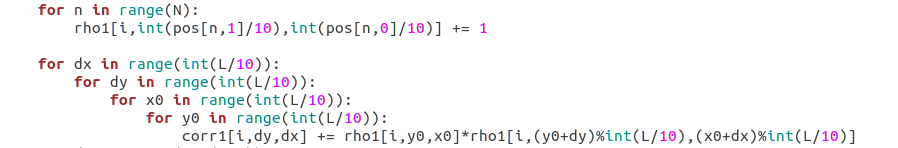
\includegraphics[scale=0.7]{corrcode.png}
	\caption{Implementierung der Korrelationsmatrix $\hat{corr_i}(\Delta x,\Delta y)$ zur Zeit $i$.}
\end{figure}

\newpage

\subsection{Selbstkorrelation}
\noindent Im folgenden wird $corr_i(0,0)$ als Selbstkorrelation eines Blocks bezeichnet, diese Größe gibt Auskunft über die die Verteilung der Walker auf die Blöcke. Dies lässt sich leicht an einem kleinen Beispiel einsehen, man stelle sich eine $3\times 3$ Matrix vor wo auf jedem Feld ein Walker sitzt, man erhält $\hat{corr}(0,0)=9$, befinden sich hingegen auf nur 3 Feldern je 3 Walker so ist $\hat{corr}(0,0)=27$. Das normieren skaliert nur die Achse, laufen Walker zusammen so steigt die Selbstkorrelation, nähern sich die Walker einer Gleichverteilung, so sinkt die Selbstkorrelation etwa auf 1, da anzunehmen ist (bei kleinen und mittleren Dichten wie sie bisher besprochen sind), dass nach einem Schritt die Walker noch Gleichverteilt sind, da sie noch nicht (indirekt über Nahrung) interagiert haben.
\\
\noindent Es wird die Selbstkorrelation für das bisherige 'Standardsystem' von 1000 Walkern auf dem $L=100$ Gitter vorgestellt. Dazu wird einmal wie oben erklärt das Gitter in 100 $10\times 10$ Blöcke unterteilt und einmal (völlig analog) in 400 $5\times 5$ Blöcke um eine feinere Auflösung zu erhalten. Leider wird die Kurve bei kleineren Blöcken (bei gleicher Sampleanzahl) weniger glatt, denn die Schwankungen sind natürlich größer, da Walker leichter am Rand des Blocks sich befinden können und somit wechseln Walker in diesem Fall leichter den Block. Eine starke Erhöhung der Anzahl von Samples ist leider (aus Gründen der Laufzeit) nicht möglich. Man erkennt jedoch trotzdem auch in dieser Variante, das Zusammenlaufen der Walker. 
\\
\noindent Man erkennt in beiden Versionen ein Ansteigen der Selbstkorrelation im streng subdiffusiven Bereich, das bedeutet, dass die Walker zusammenlaufen. Wenn der Nahrungsvorrat 'aufgegessen' ist bewegen sich die Walker wieder normal diffusiv und die Selbstkorrelation fällt wieder auf (ungefähr) 1. Im superdiffusiven Bereich bleibt die Selbstkorrelation wie zu erwarten auf (ungefähr) 1, da die Walker sich ja in kurzen Zeiten nicht sehen und nicht interagieren.
\\
\noindent Es lässt sich also sagen, dass es sich bei dem Übergang von Superdiffusion nach strenger Subdiffusion um einen Lokalisierungseffekt der Walker handelt. 
\\
\noindent Es bleibt aber zunächst offen wieso die Walker zusammenlaufen und auch der Einfluss auf das $msd$ ist unklar.

\begin{figure}[h!]
	\centering
	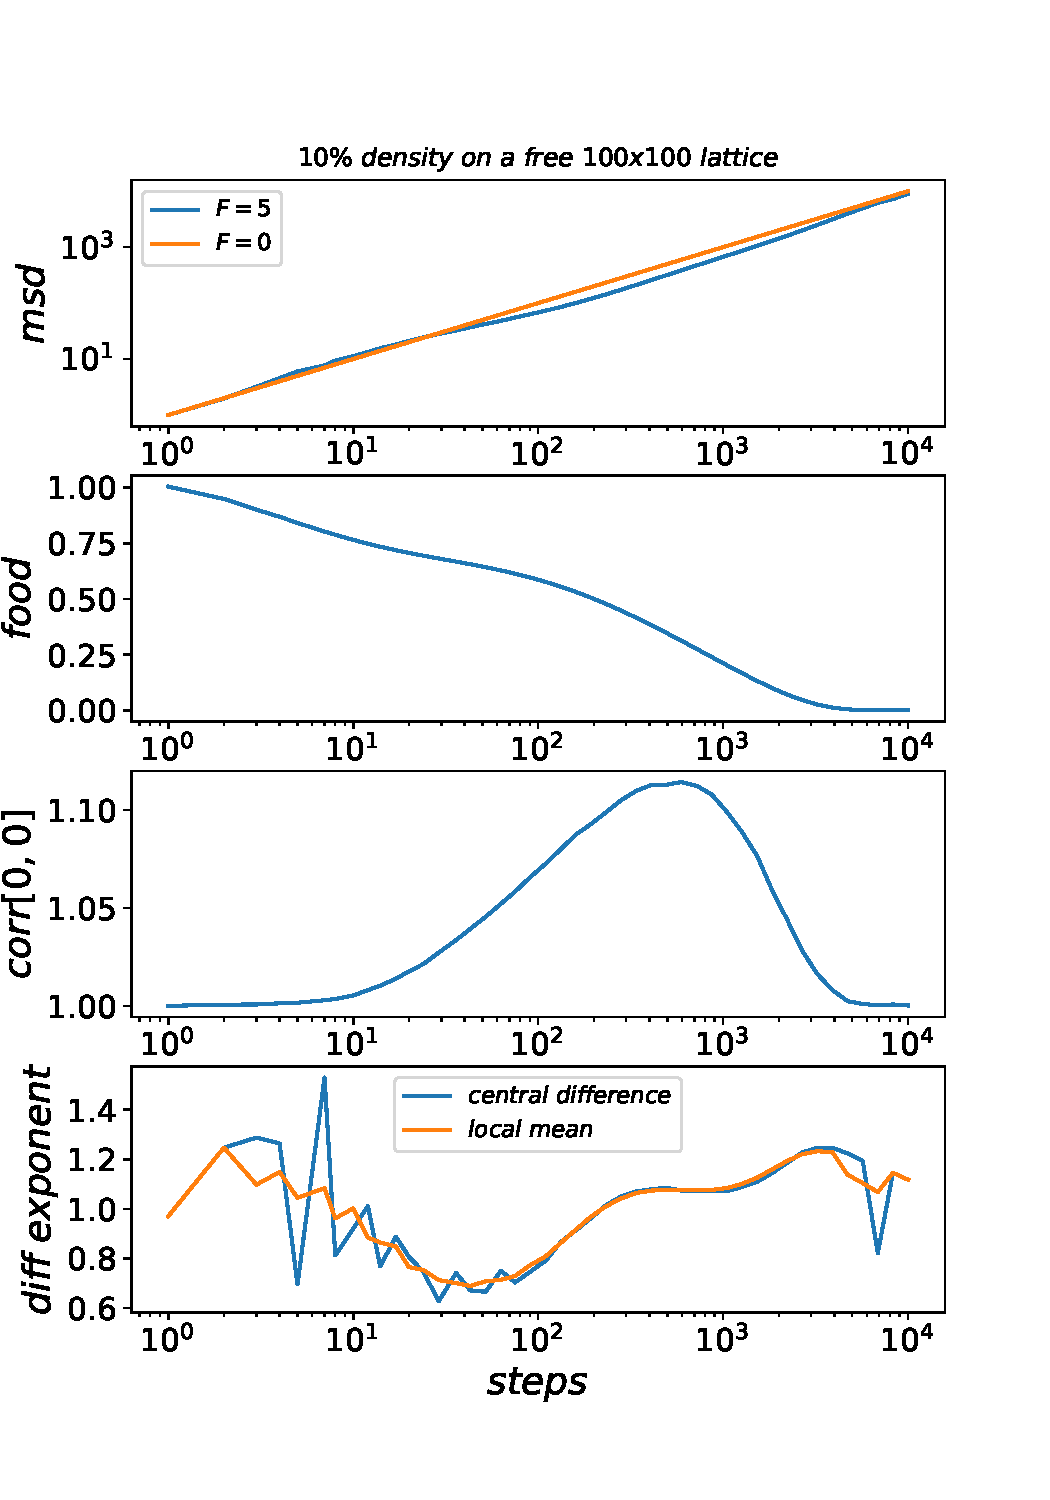
\includegraphics[scale=0.8]{corr1.pdf}
	\caption{Selbstkorrelation für $10\times 10$ Blöcke.}
\end{figure}

\newpage

\subsection{Korrelation mit benachbarten Blöcken}

In diesem Abschnitt wird die Korrelation zu benachbarten Blöcken untersucht, dabei ist es unwesentlich, ob $\Delta x$ oder $\Delta y$ zu festen Zeitschritten $t$ variiert wird, aufgrund der Symmetrie des Systems (Invarianz unter Drehungen um $\pi/2$). Es wird in nachfolgenden Plots daher stellvertretend für beide Möglichkeiten $\Delta x$ variiert.

\begin{figure}[h!]
	\centering
	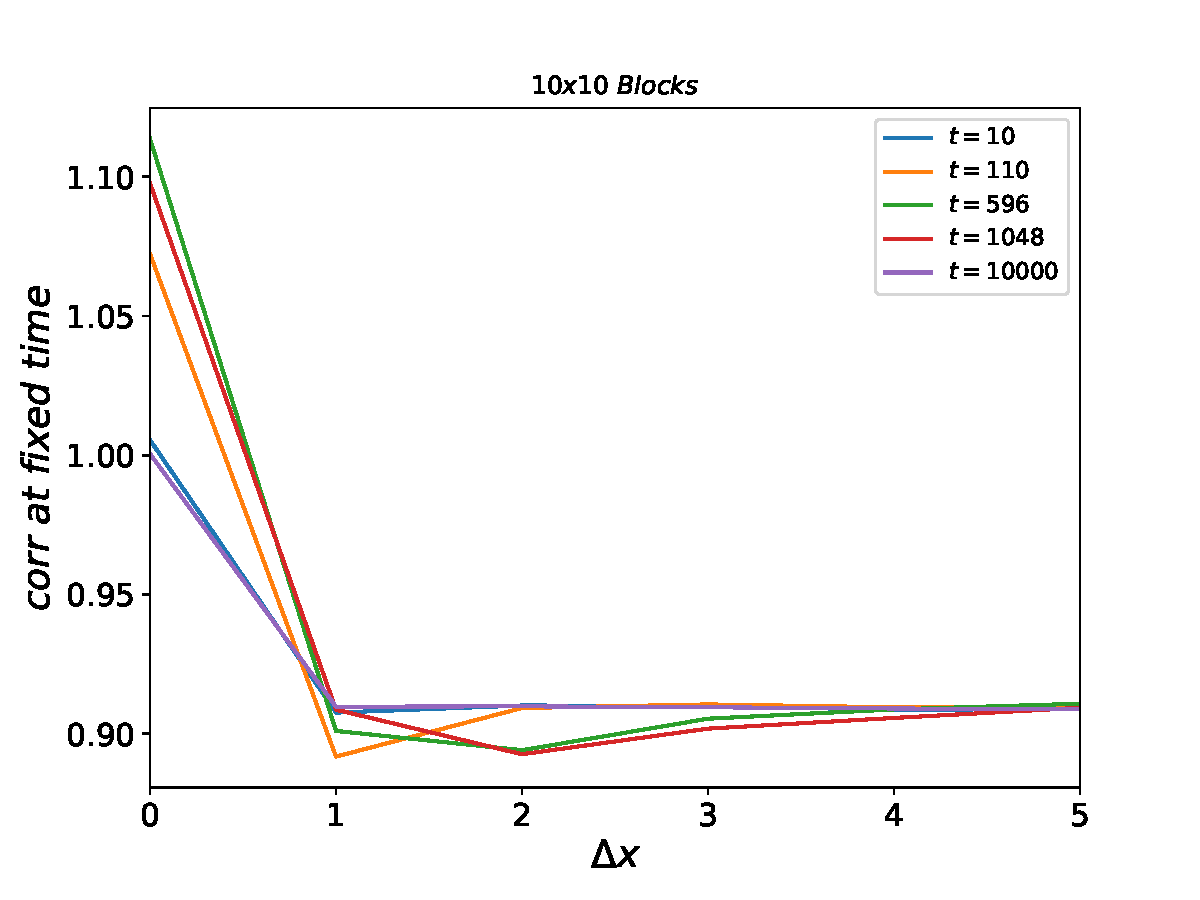
\includegraphics[scale=0.8]{corr10.pdf}
	\caption{Korrelation zu benachbarten Blöcken für eine Blockgröße von $10\times 10$.}
\end{figure}

\noindent Man erkennt, dass kurze und lange Zeiten erneut das gleiche Korrelationsverhalten haben, wie es sich nach dem vorigen Abschnitt schon vermuten lies. Wie zuvor sieht man die Steigung der Selbstkorrelation im streng subdiffusiven Bereich (also nach etwa 100 bis 1000 MC-Schritten), damit einhergehend fällt die Korrelation mit dem benachbarten Block. Man kann also sagen, dass die Teilchen aus den Nebenblocks zusammenwandern. Viele Blocks weiter (also hier 5) ändert sich die Korrelation nicht, da wie Walker nicht so weit laufen, zum Beispiel ist die Wurzel aus dem $msd$ zu $t=1048$ etwa $\sqrt{msd(1048)} \approx 30$, somit ist der Walker erst ungefähr 3 Blöcke weiter. 


\begin{figure}[h!]
	\centering
	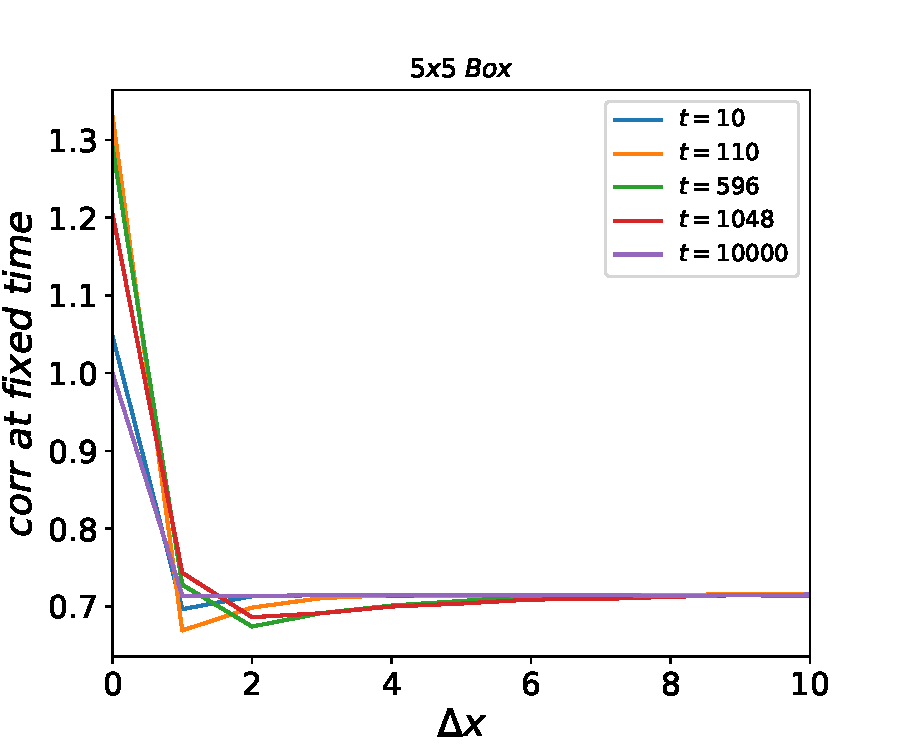
\includegraphics[scale=1]{corr5.pdf}
	\caption{Korrelation zu benachbarten Blöcken für eine Blockgröße von $5\times 5$.}
\end{figure}

\section{Autokorrelation der Schritte}
Da das $msd$ einen streng subdiffusive Bereich hat, liegt die Vermutung nahe, das die Walker 'zurückgezogen' werden zu ihren Startpunkt. Um diese Vermutung zu Untersuchen kann die folgende Korrelationsfunktion $g_{t_0}(\tau)$ gebildet werden. Es wird zuerst das (euklidische) Skalarprodukt zwischen dem Schrittvektor $\hat{e}(t_0)$ zur Zeit $t_0$ und dem Schrittvektor \break $\hat{e}(t_0+\tau)$ zur Zeit $t_0 + \tau$ eines Walkers berechnet und anschließend über alle Walker und alle Samples gemittelt, also bezeichnet $\langle \dots \rangle$ eine Ensemblemittelung. \\
\noindent Es ist demnach:
\begin{align}
g_{t_0}(\tau) = \langle \hat{e}(t_0+\tau) \cdot \hat{e}(t_0) \rangle\ .
\end{align}
Bei einem klassischen Random-Walk ist $g_{t_0}(\tau \neq 0)= 0$ für alle $t_0$ und natürlich gilt immer $g_{t_0}(\tau = 0)= 1$ denn $\hat{e}(t_0)$ ist einer der vier Einheitsvektoren $\pm \hat{e}_x,\ \pm \hat{e}_y$.
\\
Offensichtlich ist $g_{t_0}(\tau)$ positiv wenn mehr Schritte zur Zeit $t_0+\tau$ in als entgegen der Richtung des Schrittes zur Zeit $t_0$ gegangen sind und negativ anders herum. 
\\
\noindent Würden die Walker also 'zurückgezogen' werden, so würde man dies an einem negativen $g_{t_0=0}$ zu Zeiten der strengen Subdiffusion erkennen können. 

\begin{figure}[h!]
	\centering
	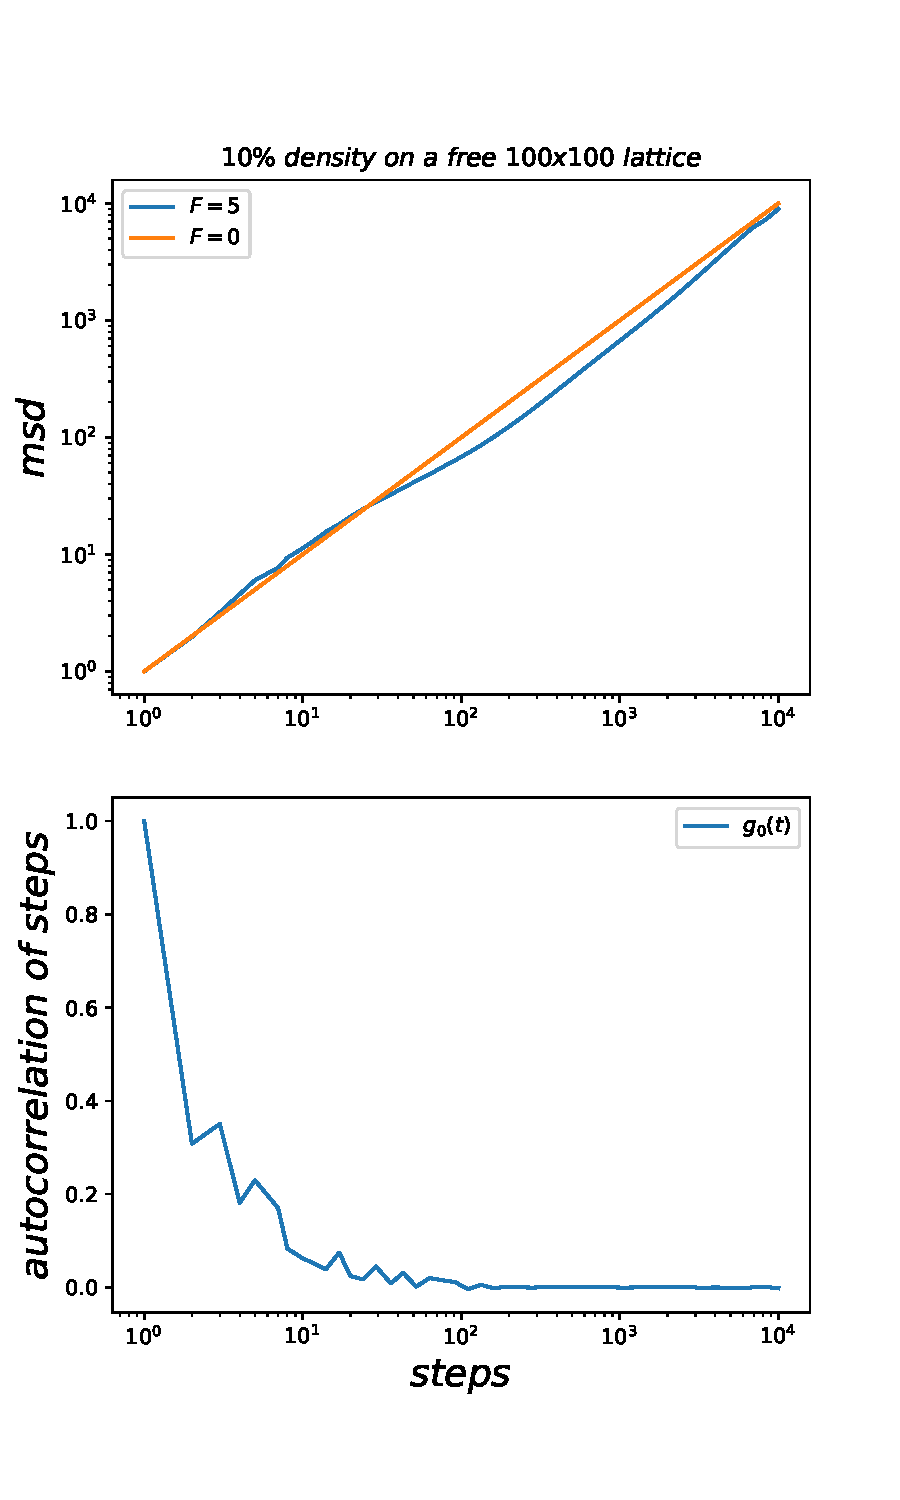
\includegraphics[scale=0.75]{autocorr.pdf}
	\caption{Autokorrelation der Schritte im Vergleich mit dem $msd$.}
\end{figure}

\clearpage

\section{'Fressspuren als Wände'}
Um zu klären, wieso das $msd$ bei $F=5$ einen streng subdiffusiven Bereich besitzt schaut man sich zunächst die Nahrungsmatrix zum Zeitpunkt $t=100$ an. Es ist zu sehen, dass die Fressspuren die Matrix in viele kleine Cluster teilt. 

\begin{figure}[H]
	\centering
	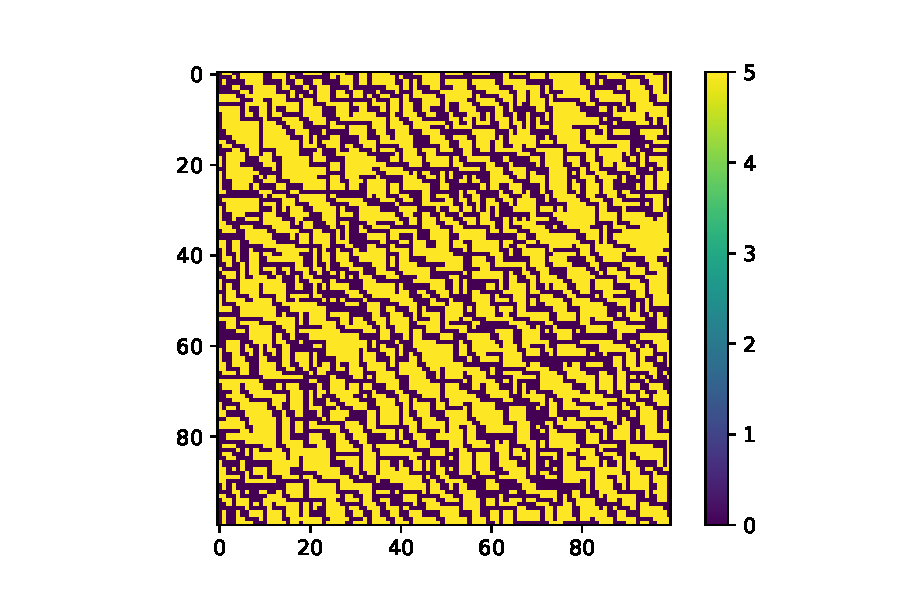
\includegraphics[scale=0.8]{usedmat.pdf}
	\caption{Nahrungsverteilung nach 100 MC-Schritten, also in der subdiffusiven Phase. Gelb = Nahrung, Schwarz = keine Nahrung}
\end{figure}


\noindent Die hungrigen Walker gehen nahezu sicher (wenn es möglich ist) auf Felder mit Nahrung: denn angenommen eins der vier benachbarten Felder enthält Nahrung und die anderen 3 nicht, so beträgt die Wahrscheinlichkeit auf das mit Nahrung besetzte Feld zu gehen gemäß Gleichung \ref{Wkeiten} $\ \frac{e^5}{e^5 + 1+ 1+1} \approx 0.98$. Somit wirken die Fressspuren wie eine Art Wand, falls Nahrung in der Nähe ist. Die Walker werden also auf die kleinen Nahrungscluster 'eingeschlossen' bis diese 'aufgefressen' sind.


\subsection{Minimalmodel eines Walkers auf einem Nahrungsquadrat}\label{minimalmodell}
Ein leicht zu verstehendes und auch leicht zu implementierendes Minimalmodell ist es einen einzelnen Walker in die Mitte eines kleinen mit Nahrung besetzten Quadrates innerhalb einer größeren Matrix zu setzen. Hier wird zum Beispiel in die Mitte einer $L=100$ Matrix ein $l=20$ Quadrat mit Nahrung belegt (das heißt auf die x und y Indices 40 bis einschließlich 59), der Walker startet bei $x_0=y_0=50$.

\begin{figure}[H]
	\centering
	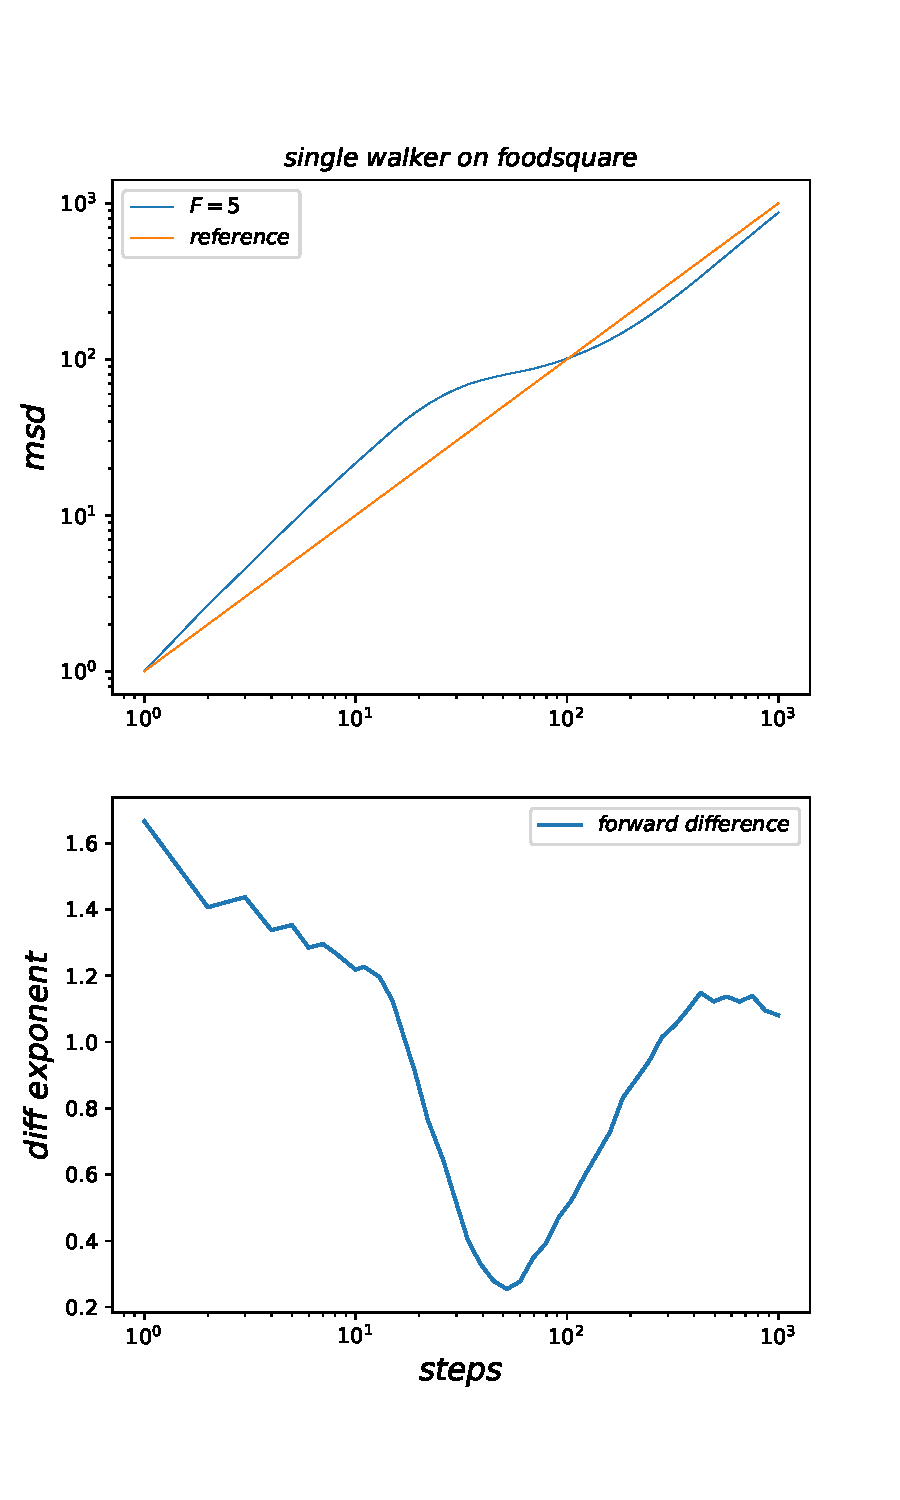
\includegraphics[scale=0.7]{single_walker_on20x20.pdf}
	\caption{Ergebniss der MC-Simulation des oben vorgestellten Minimalmodells. Es wurde über $10^5$ Samples gemittelt.}
\end{figure}


\noindent Es ist in der nachfolgenden Abbildung zu sehen, dass der Walker bei etwa $\sqrt{msd} \approx 10$ streng subdiffusiv wird, dies passt genau mit dem Erreichen von dem Rand des Nahrungsquadrat zusammen. Nach ungefähr 200 bis 300 MC-Schritten läuft der Walker wieder in fast diffusiv, da er sich 'freigefressen' hat, das Nahrungsquadrat ist nahezu leer und der Walker hat kein mit Nahrung benachbartes Feld um sich. 
\\
\noindent Zudem erkennt man an der numerischen Ableitung, beziehungsweise am daraus bestimmten Exponenten, dass das $msd$ fast konstant wird. Der (doppelte) Diffusionsexponent sinkt bis auf ungefähr $0.25$ ab, was eine sehr stark annormale Diffusion bedeutet.
\\
\noindent Das streng subdiffusive Verhalten lässt sich also auf diese Weise erklären. Da die vielen Walker auch nicht alle in gleich großen Nahrungsclustern 'eingeschlossen' sind tritt der Effekt (wie man am Vergleich der Exponenten erkennen kann) natürlich weniger stark auf.
\\
\noindent Nachfolgende Abbildungen zeigen, dass der Effekt sich (zeitlich) verschieben lässt, wenn das Nahrungsquadrat eine andere Größe besitzt. In jedem Fall ist es klar zu sehen, dass zum Zeitpunkt des Wechsels zwischen Superdiffusion nach strenger Subdiffusion der Abstand zum Rand der Nahrung etwa mit der Wurzel aus dem $msd$ übereinstimmt.
\\
\noindent Erneut (vergleiche mit Abbildung \ref{vieleF}) lässt sich die stärke des Effekts über den Parameter $F$ steuern. Dies ist einsichtig, denn je größer $F$ desto eher läuft der Walker (falls es möglich ist) auf ein zuvor unbesuchtes, also noch mit Nahrung bestücktes Feld. Im Umkehrschluss wird also die 'Fressspur' bei höherem $F$ stärker gemieden.

\begin{figure}[H]
	\centering
	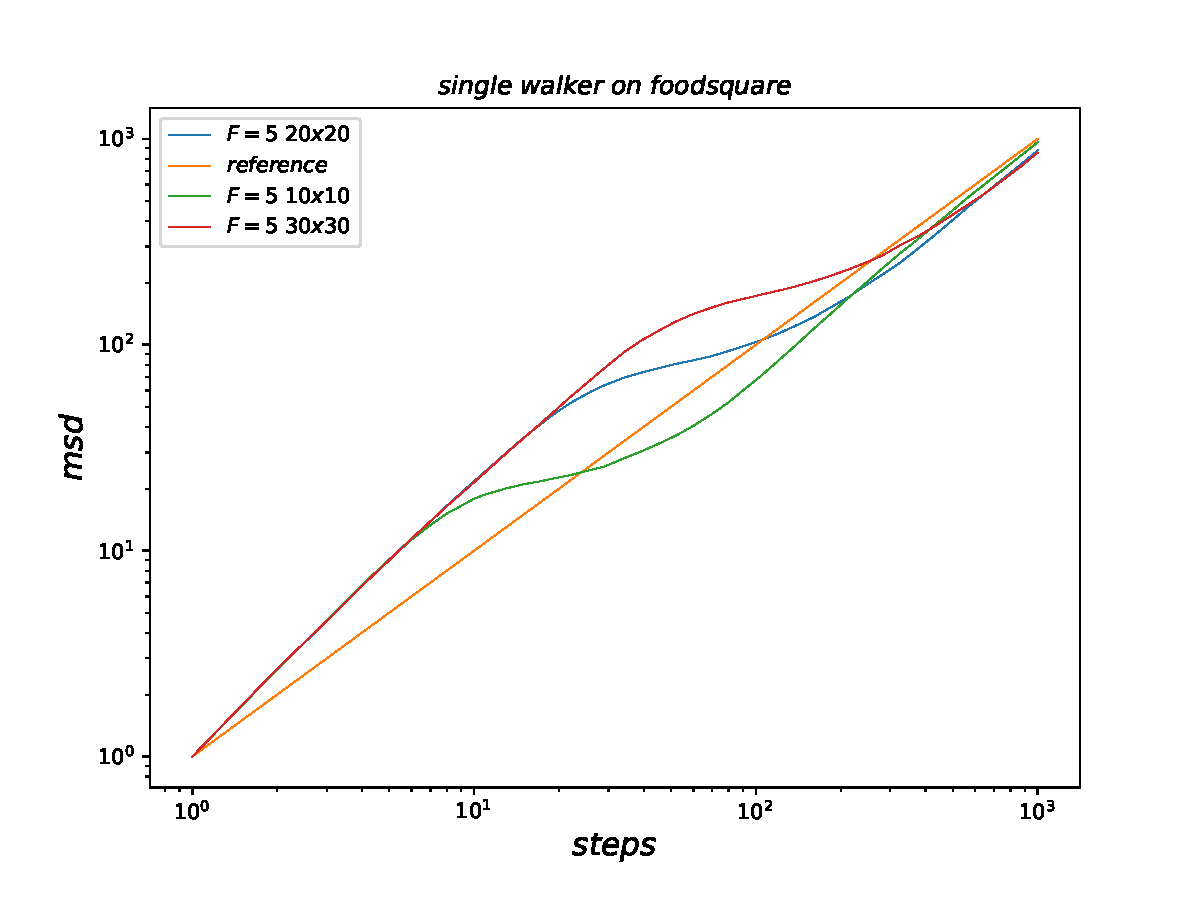
\includegraphics[scale=0.8]{abc.pdf}
	\caption{Ergebniss der MC-Simulation eines einzelnen Walkers auf Nahrungsquadraten unterschiedlicher Größe.}
\end{figure}

\newpage

\subsection{Einzelner Walker auf der Nahrungsmatrix bei fixem Startpunkt}

In diesem Unterkapitel soll das $msd$ eines einzelnen Walkers auf einer Nahrungsmatrix die vorher von vielen Walkern 'angefressen' worden ist betrachtet werden. 
Das $msd$ in der Standardkonfiguration von Boxlänge $L=100$ und $N=1000$ Walkern, sowie Nahrungsparameter $F=5$, ist nach bei $t=42$ MC-Schritten zum Beispiel im subdiffusiven Bereich. Zu diesem Zeitpunkt wird eine Nahrungsmatrix gespeichert und ich suche (durch anschauen) das Ende einer Fressspur. Dort werden die Läufe des einzelnen Walkers gestartet. 
In der nachfolgenden Abbildung sieht man die für die Simulation verwendete Matrix.



\noindent Es wird die am Punkt $x=49,\ y=65$ endende Fressspur als Startpunkt für die Simulation gewählt. Es wurde über $10^6$ Läufe gemittelt.
\\
Man sieht, dass $msd$ weißt einen 'kleinen Knick' auf an dem der Exponent der Dynamik kleiner ist als bei freier Diffusion, allerdings fällt das $msd$ nicht unter das der freien Diffusion. Das verhalten der Kurve ist jedoch ähnlich, sie steigt zunächst stark an, steigt dann deutlich wenier stark und danach steigt sie wieder stark an. Die (numerische) Ableitung und damit auch die Kurve des Diffusionsexponenten sieht daher der der vielen Walker auch ähnlich aus. Man sieht zudem, dass der Diffusionsexponent unter 1 fällt, für ein paar Schritte liegt als Subdiffusion vor. (Achtung: keine strenge Subdiffusion, da $msd$ nicht unter diffusiv fällt!)


\begin{figure}[H]
	\centering
	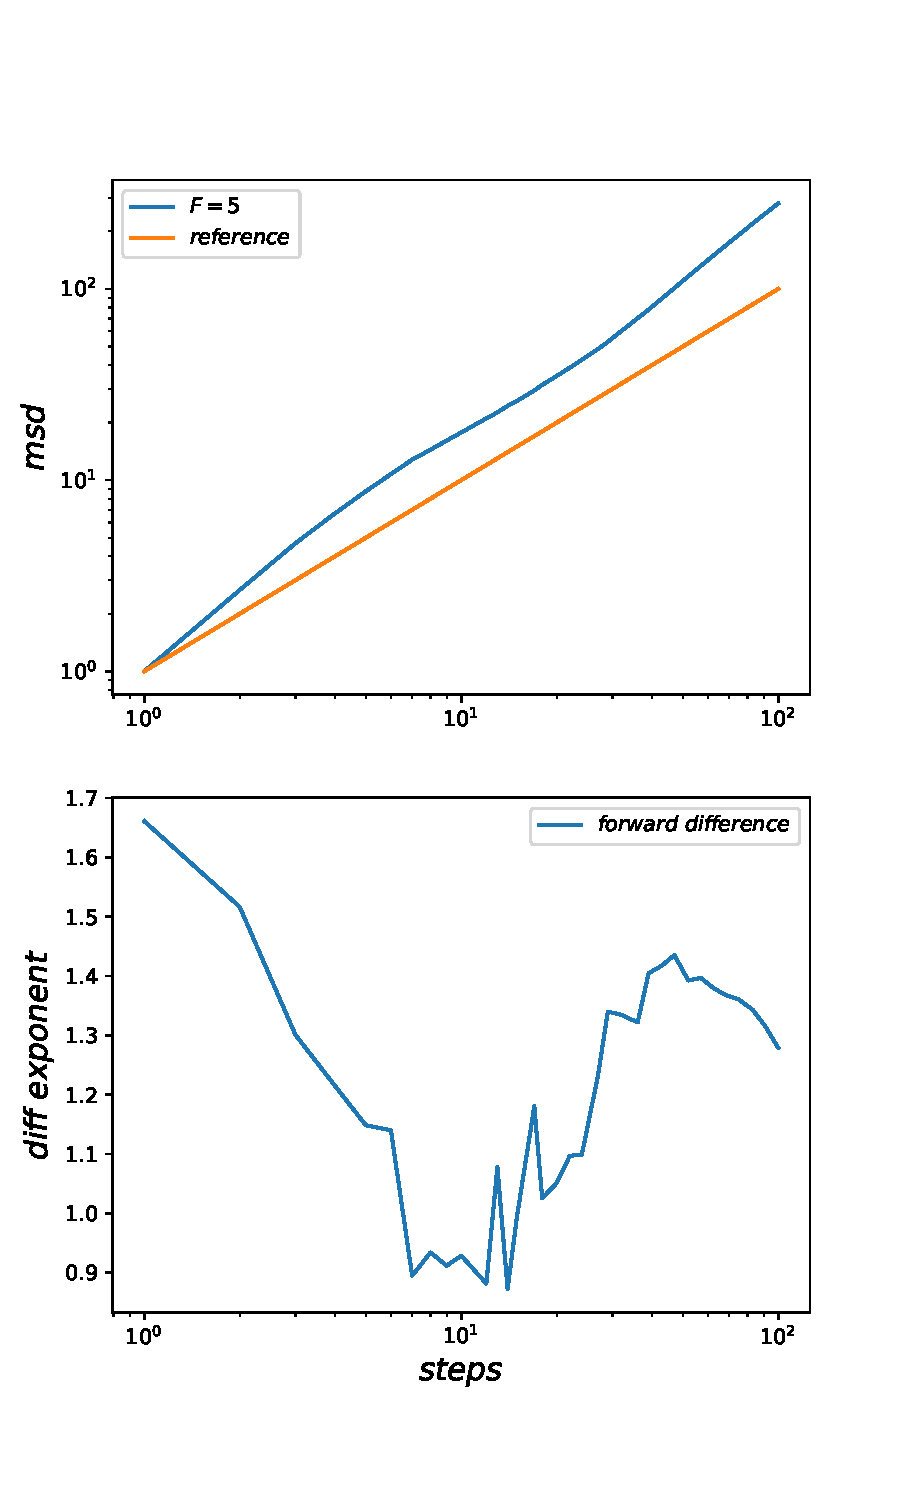
\includegraphics[scale=0.7]{single_walker_on_used_mat_nodisorderavg.pdf}
	\caption{Ergebniss der MC-Simulation eines einzelnen Walkers auf benutzter Nahrungsmatrix mit festem Startpunkt}
\end{figure}
\newpage

\subsection{Einzelner Walker auf der Nahrungsmatrix mit disorder-average}
Anders als im vorigen Unterkapitel wird nun der Startpunkt beliebig gewählt unter der Bedingung, dass von einem bereits besuchten Feld gestartet wird, dadurch wird über die Unordnung des Systems gemittelt ('disorder average'). Alternativ (oder zusätzlich) kann man auch über Nahrungsmatrizen mitteln, auch so ändert sich die Unordnung der Nahrung. 
\\
\noindent Es wird also versucht die Vielteilchendynamik auf eine Einteilchendynamik in einem 'effektiven Potential' zu übertragen. So kann herausgefunden werden ob die weitere Bewegung der anderen Random Walker auf dem bereits zerfallenen Nahrungsgitter noch den einen Walker beeinflusst.
\\
\noindent Man sieht keine Subdiffusion mehr, der Diffusionsexponent ist größer 1. Der Effekt verschwindet also durch den disorder-average. Der subdiffusive bereich war nur ein paar wenige Schritte lang. Wann die Subdiffusion eintritt ist stark von der disorder abhängig (vergleiche die unterschiedlich großen Nahrungsquadrate im Minimalmodell), mitteln wir über den Startpunkt so tritt dieser schwache subdiffusive Bereich immer zu anderer Zeit auf und mittelt sich weg.
\\
\noindent Es ist also die Bewegung der anderen Walker und die damit verbundene Veränderung der Nahrungsverteilung die diesen langen (streng) subdiffusiven Bereich hervorruft.

\begin{figure}[H]
	\centering
	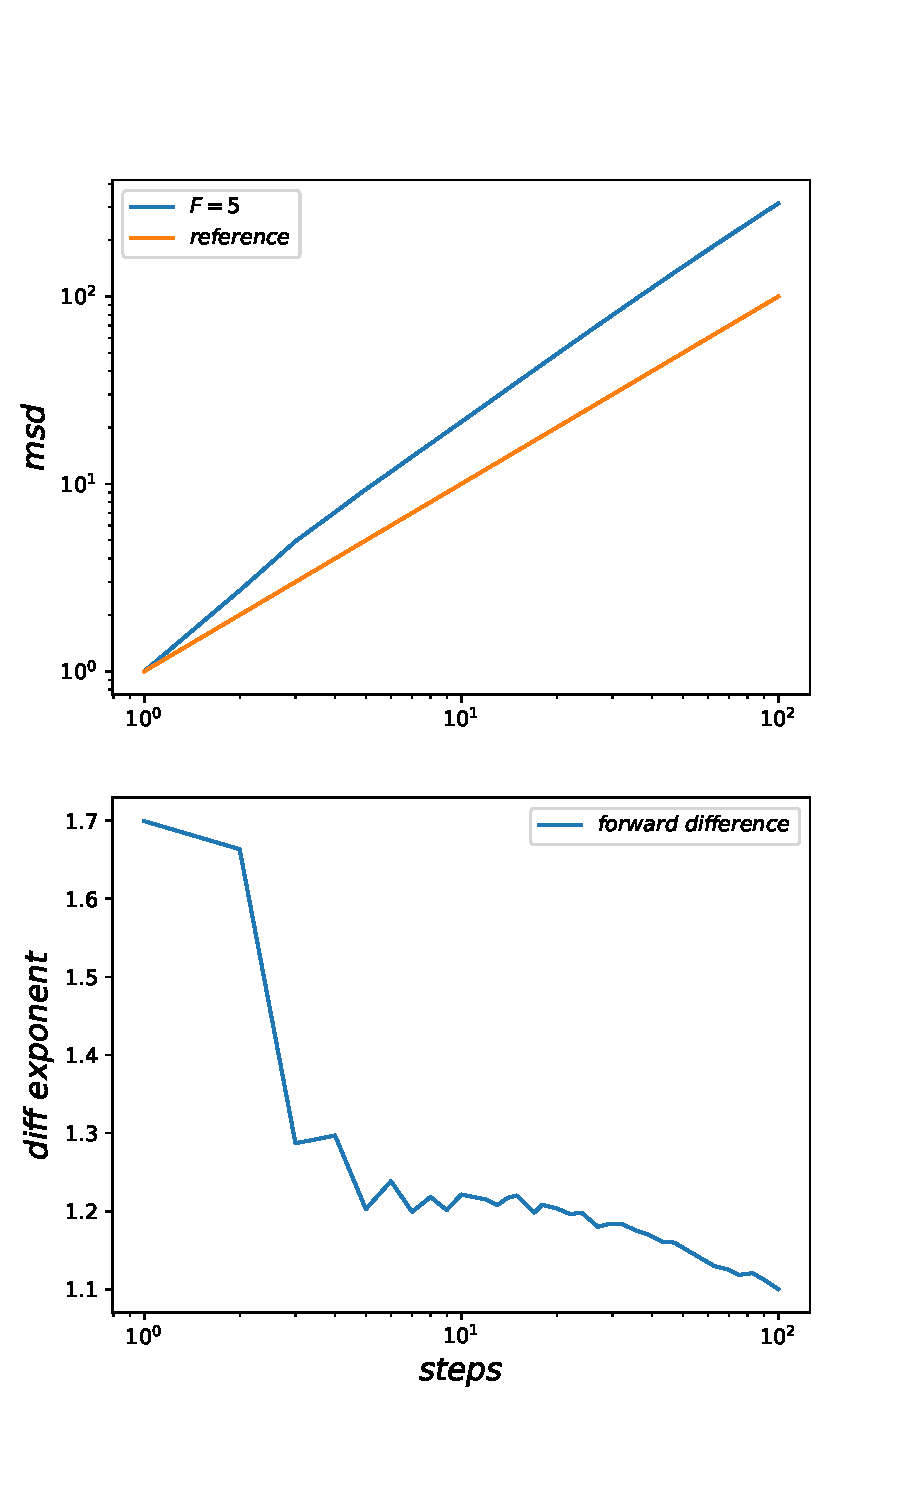
\includegraphics[scale=0.8]{single_walker_on_used_mat_disorderavg.pdf}
	\caption{Ergebniss der MC-Simulation eines einzelnen Walkers auf benutzter Nahrungsmatrix mit zufälligem zuvor besuchten Startpunkt}
\end{figure}

\newpage

\section{Unterschiedliche Walkerdichten und ihr Effekt auf die Dynamik}
In dem vorigen Abschnitt \ref{minimalmodell} wurde der Einfluss unterschiedlich großer Nahrungsquadrate auf die Dynamik des einzelnen Walkers gezeigt. Aus diesem Ergebniss kann man raten, dass eine höhere Dichte an Random Walkern einen ähnlichen Effekt auf die Vielteilchendynamik hat wie ein kleineres Nahrungsquadrat auf die Einteilchendynamik im Minimalmodell, denn je mehr Walker auf der Nahrungsmatrix sitzen, desto schneller und und kleinteiliger zerfällt das Nahrungsgitter. 
\\
Man erwartet also, das bei steigender Dichte das streng subdiffusive Verhalten nach weniger Schritten eintritt. Naiv ist aber nicht klar, ob die stärke des Effektes von der Walkerdichte abhängig ist, also ob der Diffusionsexponent unterschidlich weit sinkt oder nicht.
\\
\noindent
Die nachfolgende Grafik zeigt die Simulationsergebnisse ($msd$ und Diffusionsexponent) bei den Walkerdichten 5\%, 10\%, 20\% und 50\% auf der $100 \times 100$ Nahrungsmatrix, es wurde über 2000, 1000, 500, 200 Läufe gemittelt um immer über $10^6$ einzelne $msd$ zu mitteln.
\\
\noindent Die Simulationsergebnisse bestätigen eindeutig, dass der Eintritt der strengen Subdiffusion mit der Dichte in oben vermuteter Weise zusammenhängt. Zudem lässt sich auch am Minimum des Diffusionsexponenten (numerisch bestimmt mit der 'forward-differnence' Methode) eine Tendenz erkennen: mit steigender Walkerdichte senkt sich das Minimum im Diffusionsexponenten nach unten. Die stärke der Subdiffusion scheint also (in dem hier simulierten Bereich mittlerer Dichten) mit steigender Dichte zuzunehmen.

\begin{figure}[H]
	\centering
	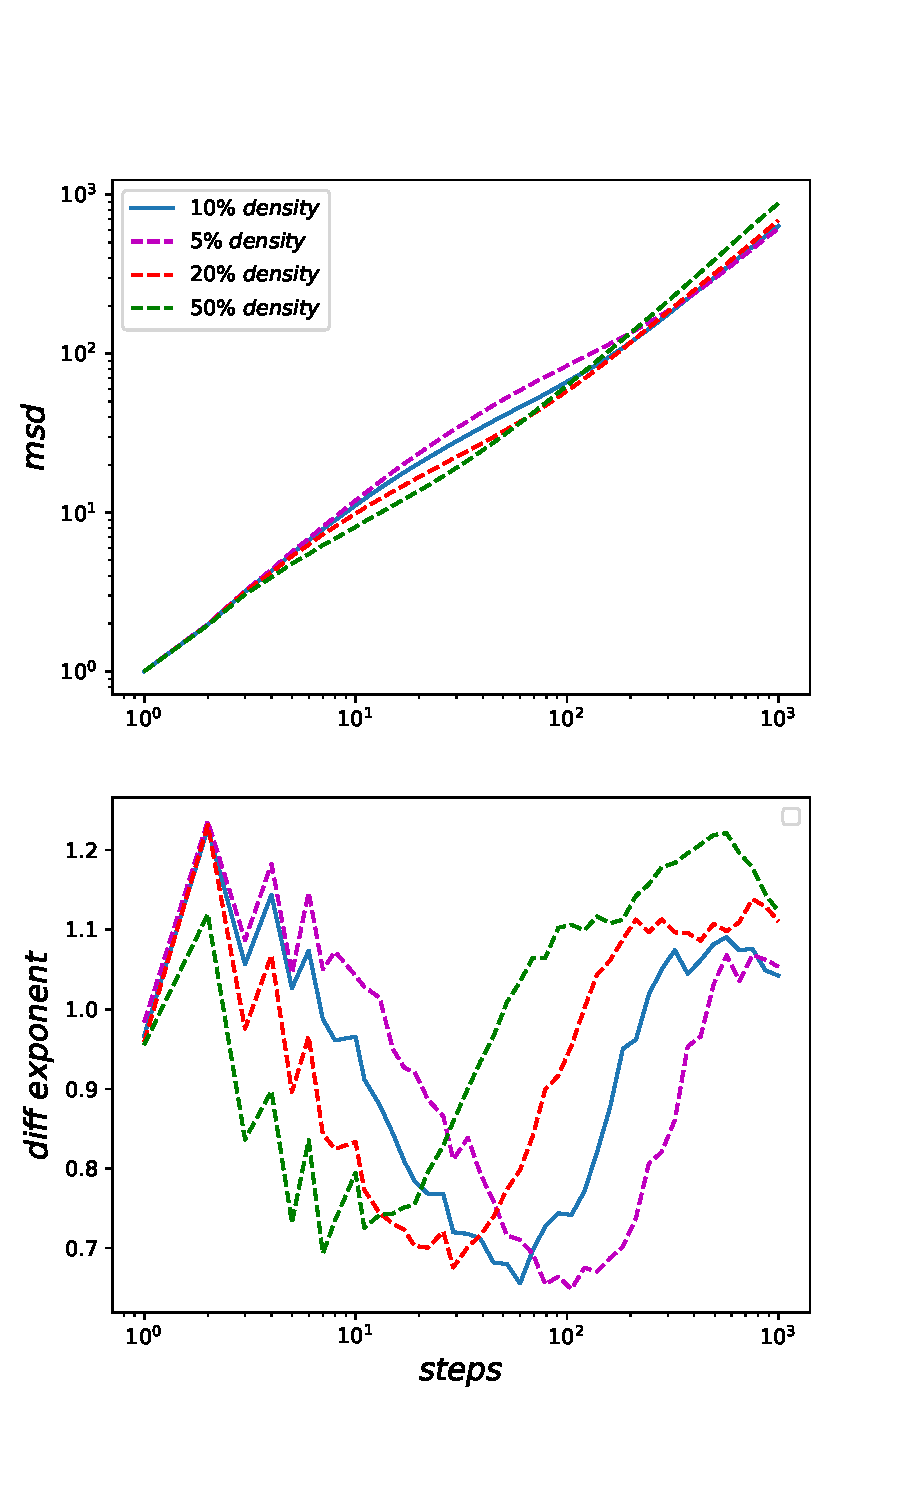
\includegraphics[scale=0.8]{alldens.pdf}
	\caption{Ergebniss der MC-Simulation bei unterschiedlichen Walkerdichten, es wurde in allen Kurven über $10^6$ einzelne $msd$ gemittelt.}
\end{figure}

\newpage
\chapter{Eindimensionales Modell vieler hungriger Walker}

\section{Mean Squared Displacement}

Um die bisherige Idee, dass die Ränder der verbliebenen Nahrungscluster die Dynamik in ein subdiffusives Regime bringen zu untermauern wird ein eindimensionales Modell betrachtet. In diesem Fall gibt es dementsprechend keine (wirklichen) Ränder, da diese nulldimensional sind, das Ablaufen eines Randes wie das Minimalmodell aus dem vorherigen Kapitel nahelegt ist daher nicht möglich. 
\\
Für die Simulation wird der gleiche Code wie bisher verwendet, also wird ebenfalls gleichzeitig und nach der selben Wahrscheinlichkeitsberechnung gezogen. 
\\
Klar ist, dass nach sehr langen Zeiten das $msd$ auf der Diffusionskurve ($F=0$) sein muss, da alle Nahrung weggessen ist und damit die Walker keine interaktion mehr haben und alle einen normalen eindimensionalen Random-Walk ausführen.
\\
Ebenfalls ist zu erwarten, dass am Anfang der Simulation die Walker stark superdiffusiv laufen müssen (bei $F=5$), da sie nahezu deterministisch in die Richtung des ersten Schrittes laufen müssen, denn es ist $\frac{e^5}{e^5 + 1} \approx 0.99$. 
\\
Kuezzeit- und Langzeitverhalten müssen daher mit dem zweidimensionalen Modell übereinstimmen, spannend ist also wie das verhalten auf mittlerer Zeitskala ist. Die entscheidende Frage lautet also: Gibt es ein subdiffusives Regime, in dem das $msd$ (bei $F=5$) unter der Diffusionskurve liegt? 

\begin{figure}[H]
	\centering
	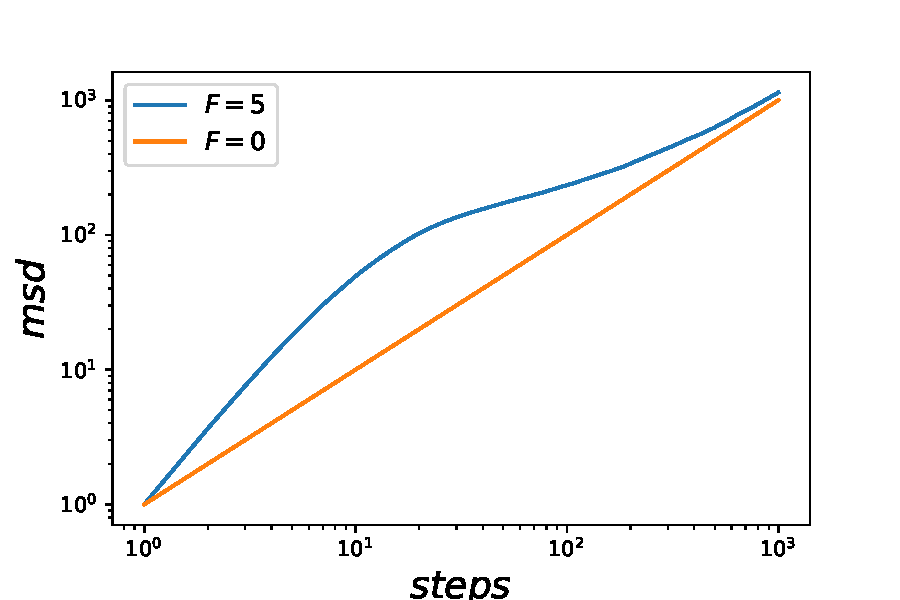
\includegraphics[scale=0.85]{onedmsd.pdf}
	\caption{Ergebniss der MC-Simulation des eindimensionalen Modells. Es wurde über 100 Läufe, also $10^4$ Samples gemittelt.}
\end{figure}

\newpage

\noindent Um Antwort auf diese Frage zu erhalten schaut man sich das Simulationsergebnis in der kommenden Abbildung an. Es gibt kein subdiffusives Regime, sondern nur ein superdiffusives zu Anfang, welches nach verschwinden der Nahrung sich auf die normale Diffusionskurve (von oben) anpasst.

\section{Autokorrelation der Schritte im eindimensionalen Modell}
Neben dem $msd$ kann erneut die Autokorrelation der Schritte $g_{t_0}(\tau)$ betrachtet werden. Aus dieser Größe kann man ablesen, wie stark der Schritt zur Zeit $t_0 + \tau$ mit dem Schritt zur Zeit $t_0$ korreliert ist.
\\
\noindent Es lässt sich eine längere Korrelation zum ersten Schritt vermuten, da bis zum erreichen der Fressspur eines benachbarten Walkers die Schritte nahezu deterministisch in die Richtung des ersten Schrittes erfolgen.
\\
\noindent In dem Plot der Autokorrelation der Schritte sieht man ganz deutlich, das der zweite Schritt noch sehr stark zum ersten Schritt korreliert ist. Dies ist im zweidimensionalen Modell nicht so gewesen. Die Erklärung dafür ist einfach, in zwei Dimensionen hat der Walker nach dem ersten Schritt (in den meisten Fällen bei 10\% Dichte) 3 Felder neben sich mit Nahrung die gleich Wahrscheinlich besucht werden, im eindimesionalen Fall nur ein Feld (das wo der Walker nicht her kommt) und daher ist die Korrelation zu Beginn stärker. 
\\
Dadurch ist auch klar, wieso das $msd$ zu Beginn stärker superdiffusiv ist.


\begin{figure}[h!]
	\centering
	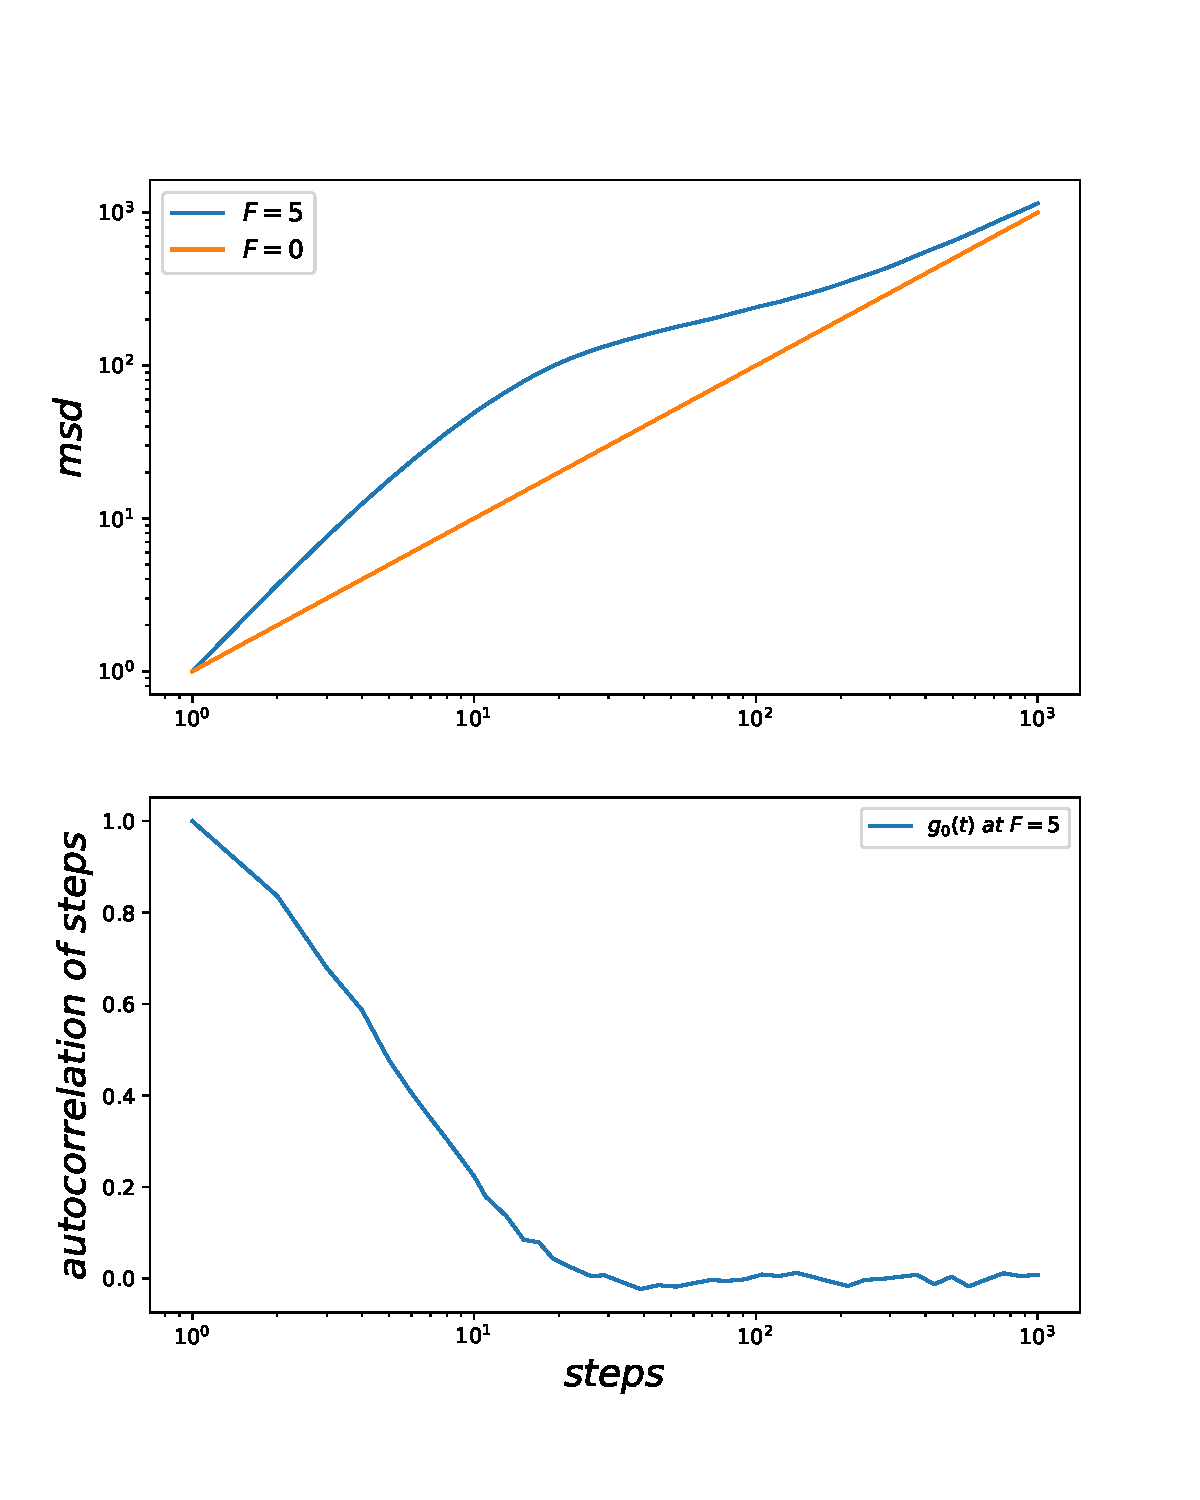
\includegraphics[scale=0.7]{onedescp.pdf}
	\caption{Autokorrelation der Schritte des eindimensionalen Modells. Es wurde über 100 Läufe, also $10^4$ Samples gemittelt.}
\end{figure}





\chapter{Viele Random-Walker auf dem perkolierenden Cluster mit Nahrung (2D)}
In diesem Kapitel wird die Dynamik vieler 'hungriger' Random Walker auf dem perkolierenden Cluster untersucht. Es wird also das 'Clearing out a Maze' Paper auf viele Walker erweitert. Wie zuvor besteht zwischen den Walkern keine direkte Interaktion, sondern nur indirekt über 'wegfressen' der Nahrung.
\\
\noindent Auf dem freien Cluster wurde gefunden, dass die Dynamik nach einem superdiffusiven Regime zu Beginn in ein streng subdiffusives Regime wechselt (d.h. der Diffusionsexponent $2\nu$ ist kleiner 1 und das $msd$ liegt unter dem der freien Diffusion). Das $msd$ nähert sich also auf lange Zeiten dem der freien Diffusion ($F=0$) von unten an.
\\
\noindent Auf dem perkolierenden Cluster gibt es zwei Vergleichskurven, der einzelne Walker mit Nahrung auf dem perkolierenden Cluster ('Clearing out a Maze') und der Fall $F=0$ also die anormale Diffusion auf dem perkolierenden Cluster ($\nu \approx 0.347$ in zwei Raumdimensionen).
\\
\noindent Zu beachten ist, dass der perkolierende Cluster immer unterschiedlich groß ist und daher unterschiedlich viele Walker für die gleiche Dichte benötigt werden. Hier wird bei der so errechneten Anzahl der Walker immer abgerundet (mittels der int()-Funktion in Python3).









\bibliographystyle{plain}
\bibliography{references.bib}

\end{document}